%!TEX root = ../../super_main.tex

\section{Participant Interaction}
When opening the mobile application, the participant is presented with an initial, as seen in \figref{fig:initial_screen}. The idea with this screen is to welcome the participant to the application. Currently, it does not supply the participant with much information, but one could imagine that this view would, in future iterations, provide the participant with usable information, such as progress in the current campaign, clarification of what concepts and principals the participants must know. This screen could possibly also contain some motivational factor, provided by customers. e.g. a ``prize'' for participation.

\todo[inline]{Skriv at vi bruger Google Material Design som udgangspunkt. Så har vi nogle ``standard'' elementer og principper at gå ud fra, så vi slipper for at opfinde den dybe tallerken}

% Initial screen
\begin{figure}[!htbp]
\begin{subfigure}[!t]{.48\textwidth}
  \centering
  
\includegraphics[width=.7\linewidth]{mockups/homepage}
  \caption{Mockup.}
  \label{fig:mockup_initial_screen}
\end{subfigure}%
\begin{subfigure}[!t]{.52\textwidth}
  \centering
  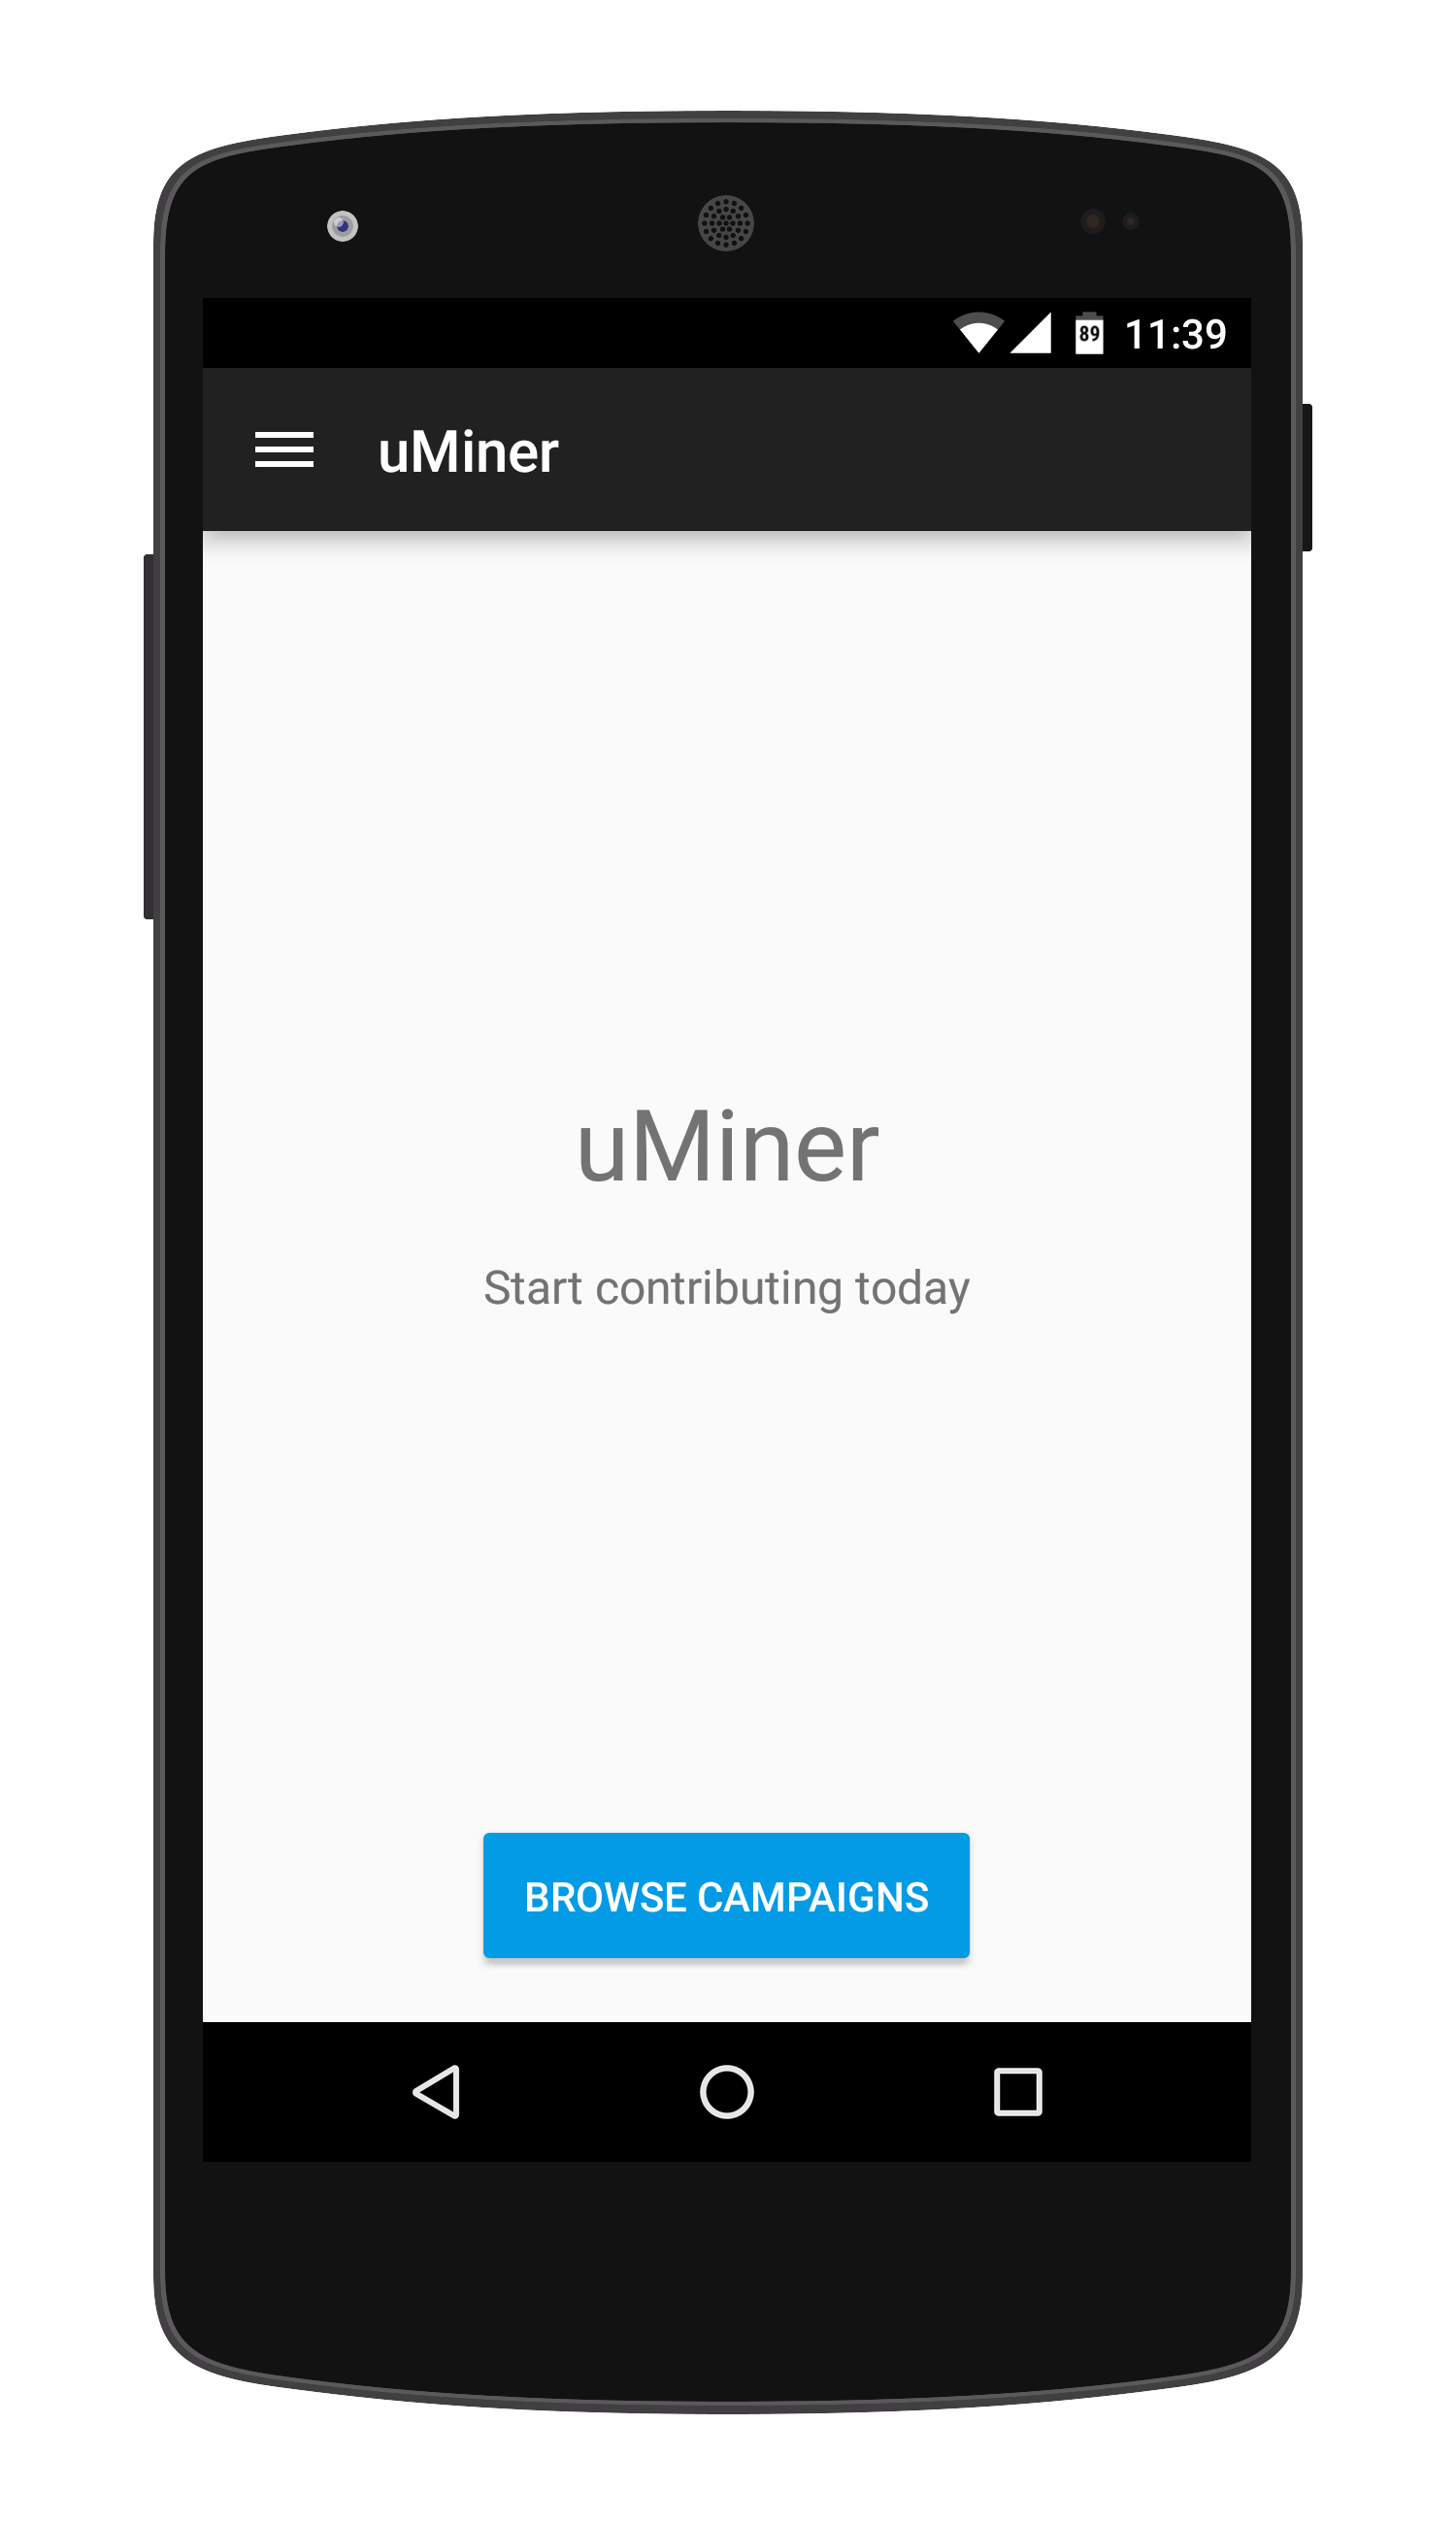
\includegraphics[width=.73\linewidth]{user_interfaces/client_uminer_home_with_phone}
  \caption{Implementation.}
  \label{fig:implementation_initial_screen}
\end{subfigure}
\caption{Initial screen of the Application.}
\label{fig:initial_screen}
\end{figure}
\FloatBarrier

To navigate to other views in the application, the participants must either use the drawer menu displayed in \figref{fig:navigation} or the \emph{browse campaigns}-button in the initial view. The navigation menu contains three elements, which will each take the participant to different parts of the application.

\begin{description}
	\item[\emph{Current campaign}] redirects the participant to a campaign specification view, as seen in \figref{fig:public_campaigns}, displaying more information about the campaign that they are currently contributing to. If the participant have not yet joined a campaign, a message will briefly be displayed on the screen, informing the participant about this.
	\item[\emph{Browse campaigns}] redirects the participant to a view containing brief information about all of the publicly available campaigns.
	\item[\emph{Join specific}] redirects the participant to a view, as seen in \figref{fig:specific_campaign}, where he/she can search for a specific campaign by providing a campaign identifier.
\end{description}

% Navigation
\begin{figure}[!htbp]
\centering
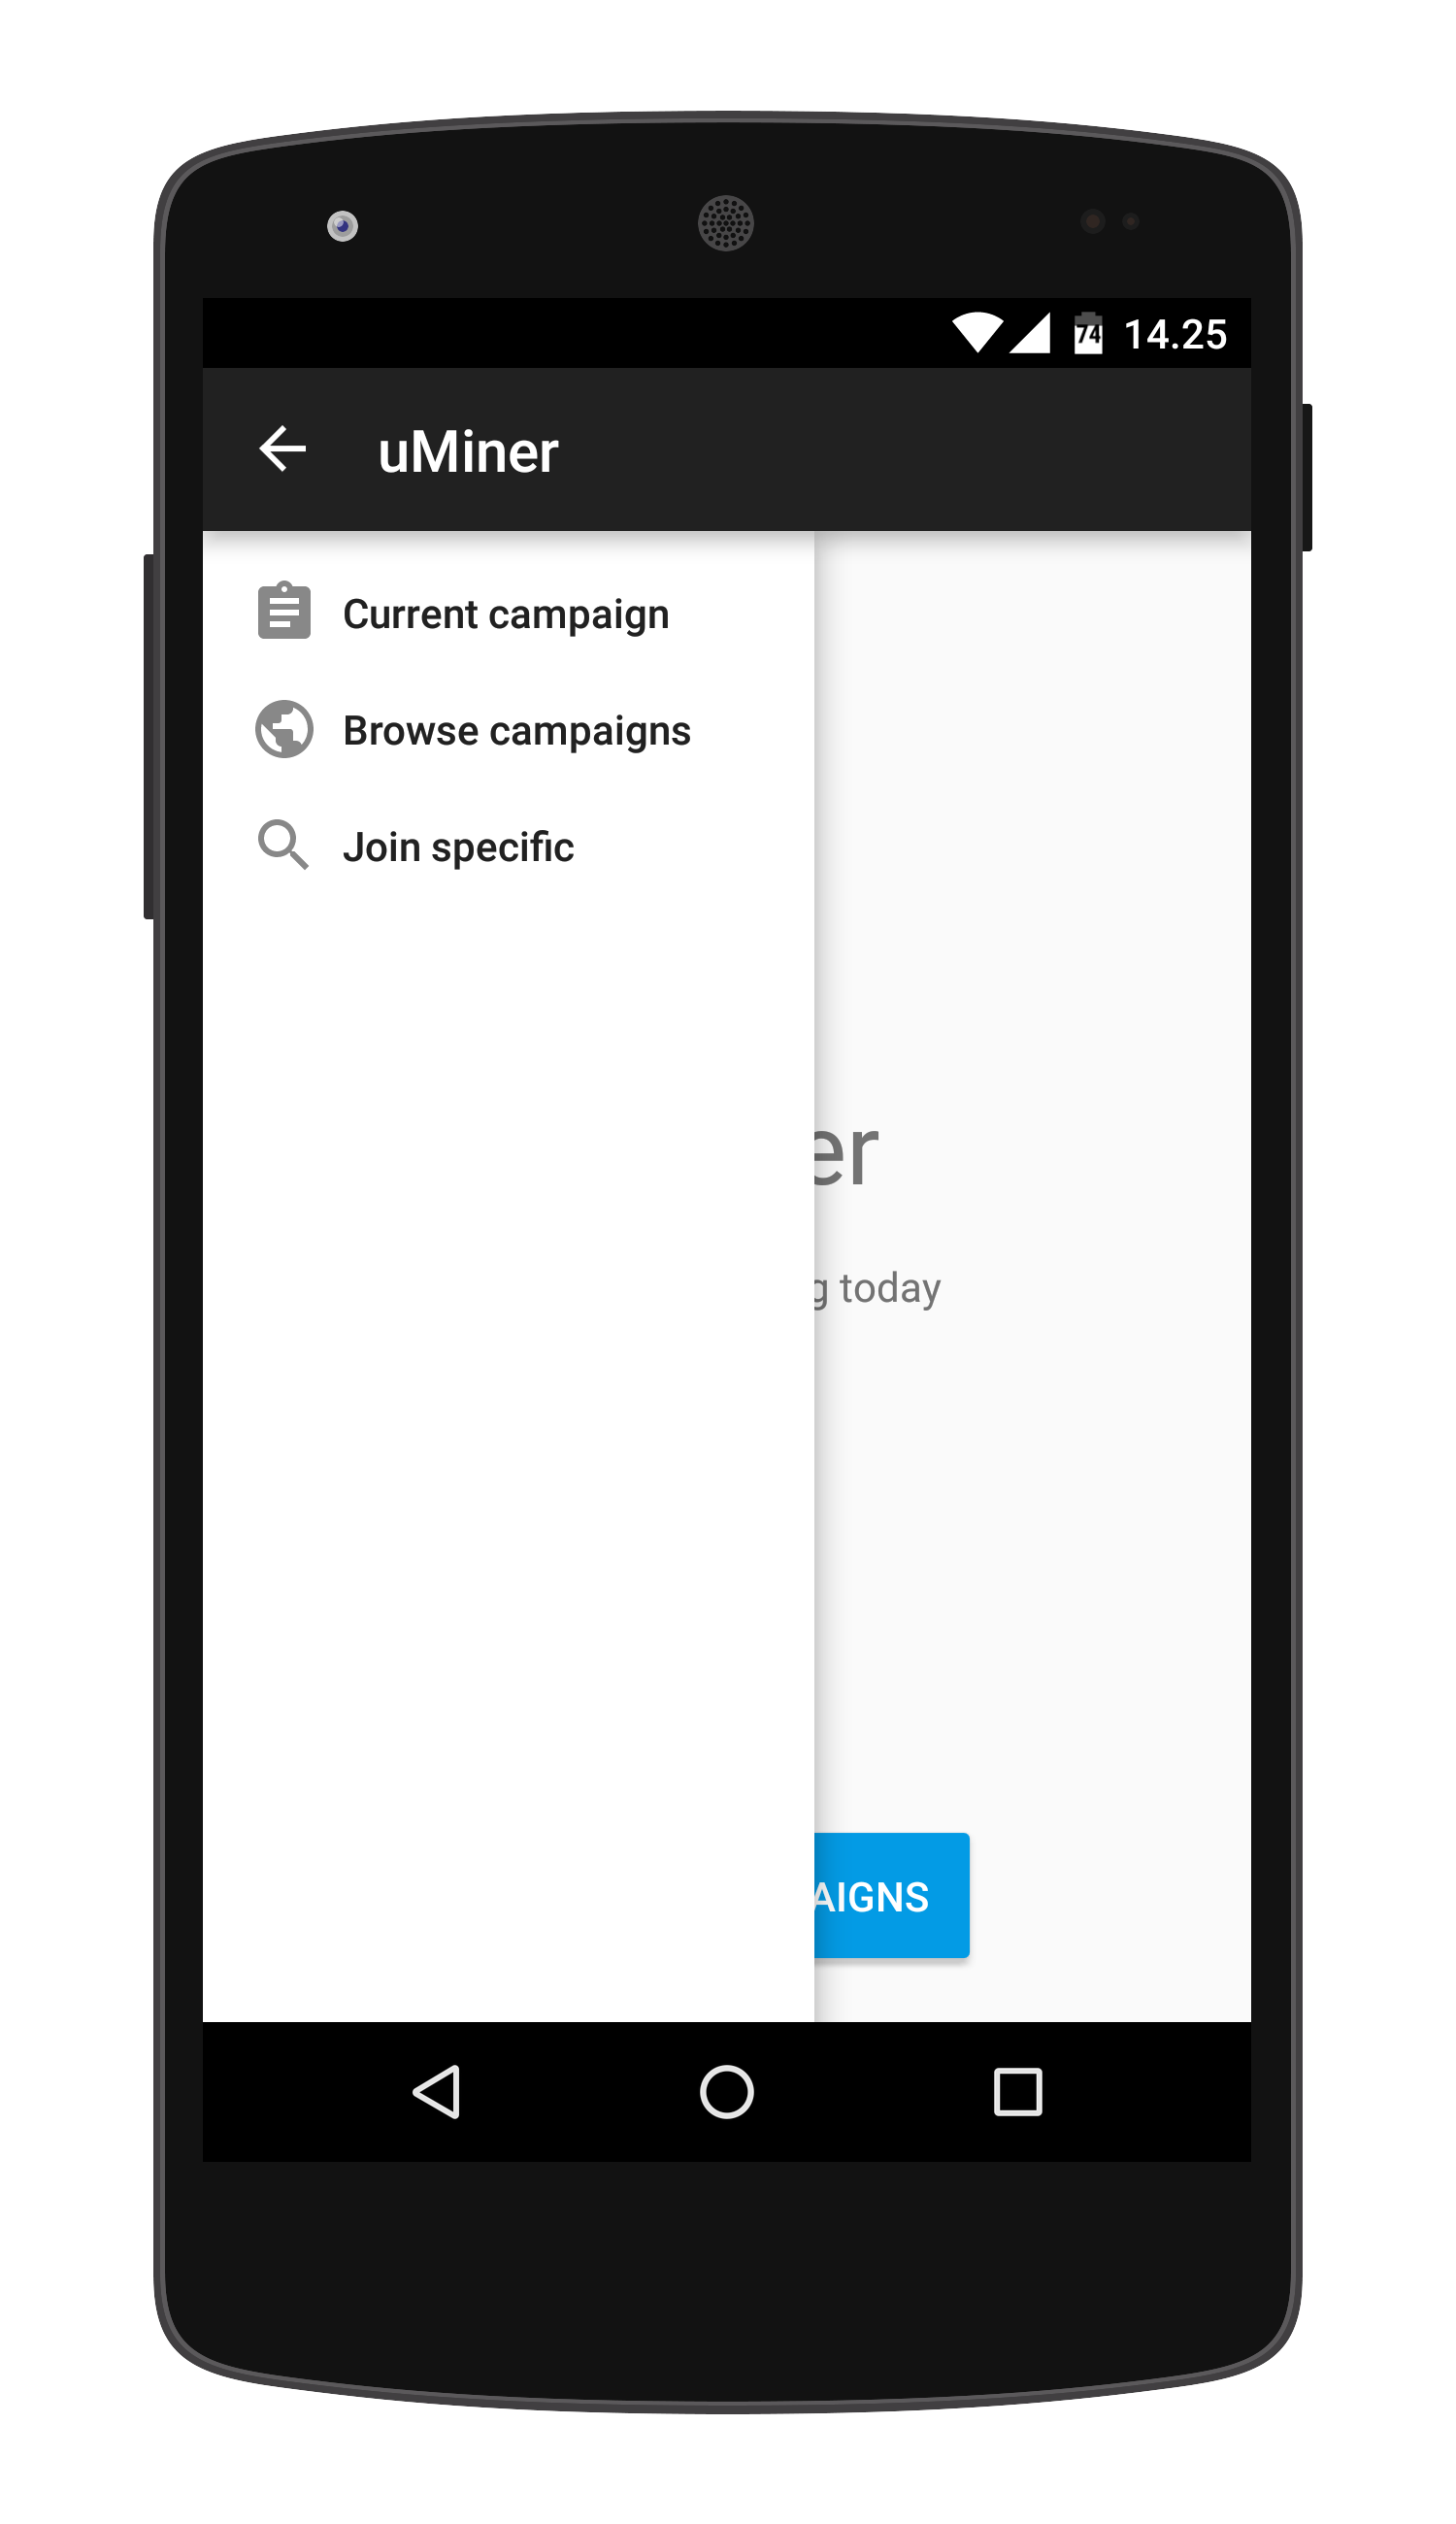
\includegraphics[width=.35\linewidth]{user_interfaces/client_drawer_menu_with_phone}
\caption{Navigation through the application.}
\label{fig:navigation}
\end{figure}
\FloatBarrier

\subsection{Browsing Campaigns}
If a participant wants to contribute to a campaign, they may browse the publicly available campaigns. This can be done through the view seen in \figref{fig:public_campaigns}. Here, all campaigns are listed displaying the title of the campaign along with the creator of the campaign. If the participant wishes to know more about a specific campaign, he/she can press it and be redirected to a view similar to the one seen on \figref{fig:campaign_specification}. The view furthermore informs the participants about the possibility to join a specific campaign by pressing the the bottom-most button, which will always be visible regardless of how far the participant scrolls in the list. By pressing this button, the participant will be redirected to the view showed in \figref{fig:specific_campaign}.

% Publicly available campaigns
\begin{figure}[!htbp]
\begin{subfigure}[!t]{.48\textwidth}
  \centering
  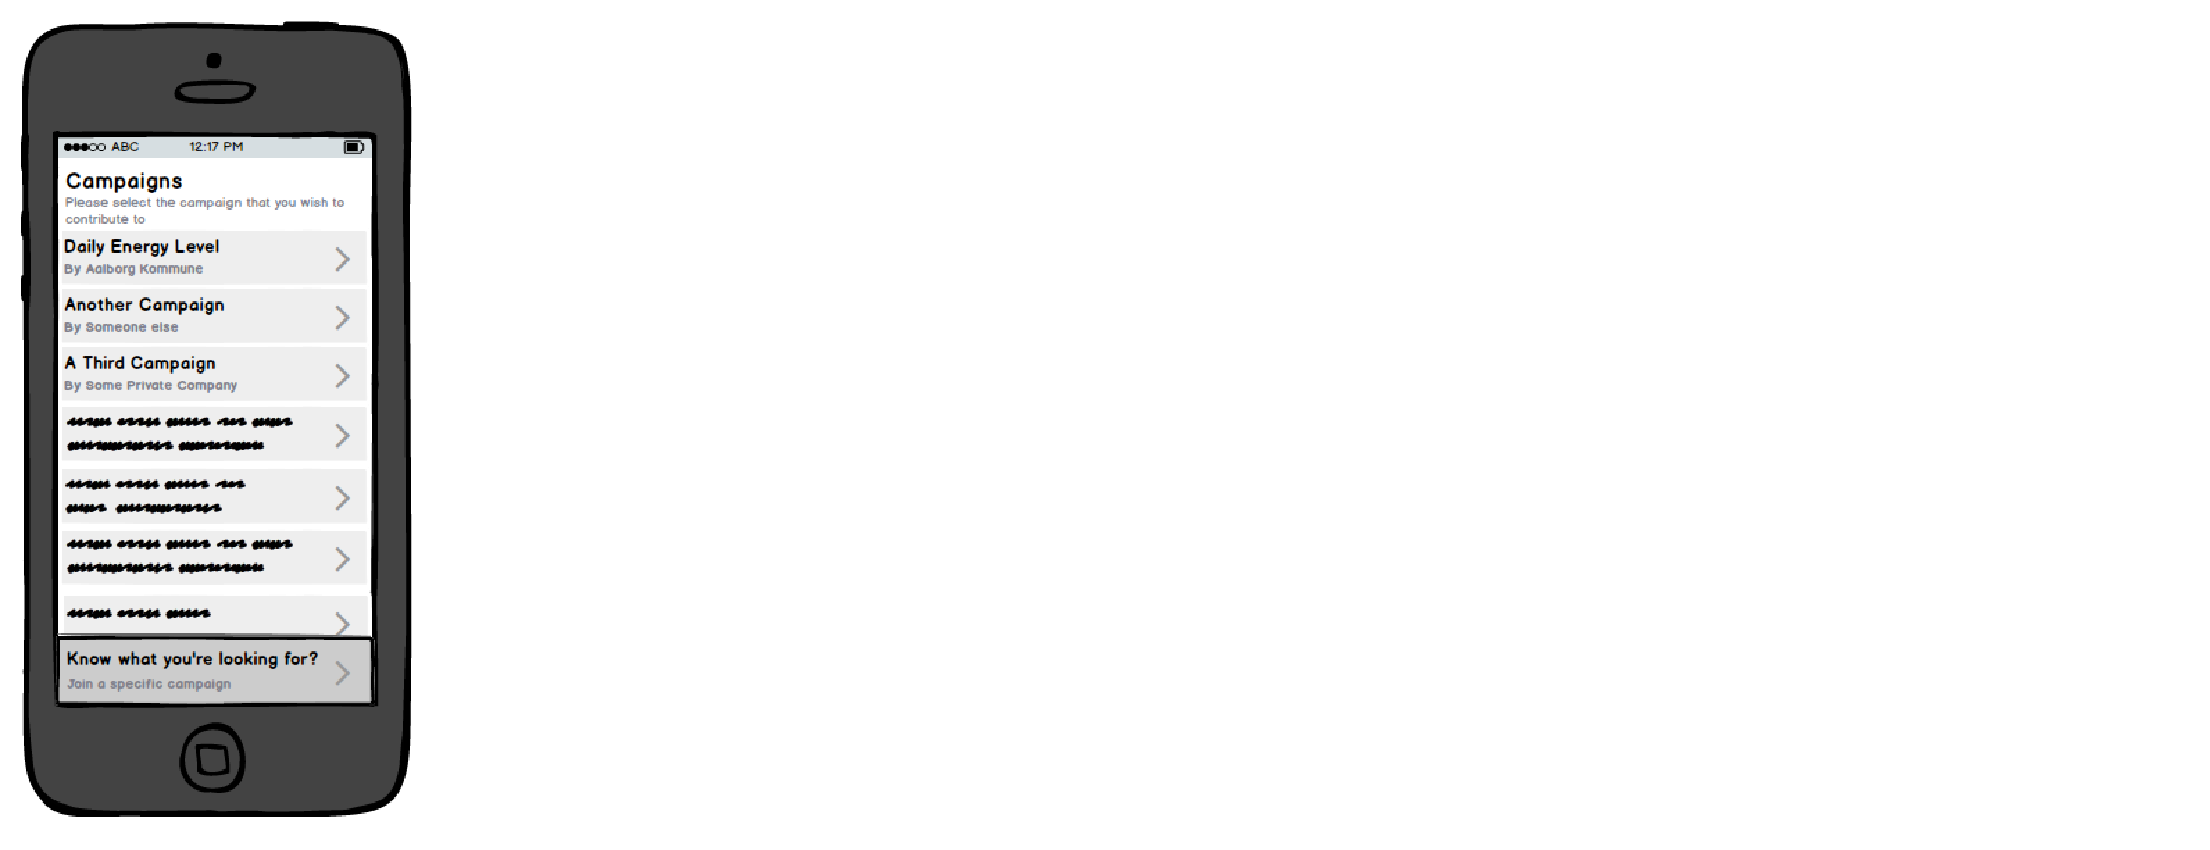
\includegraphics[width=.7\linewidth]{mockups/campaigns_list}
  \caption{Mockup.}
  \label{fig:mockup_public_campaigns}
\end{subfigure}%
\begin{subfigure}[!t]{.52\textwidth}
  \centering
  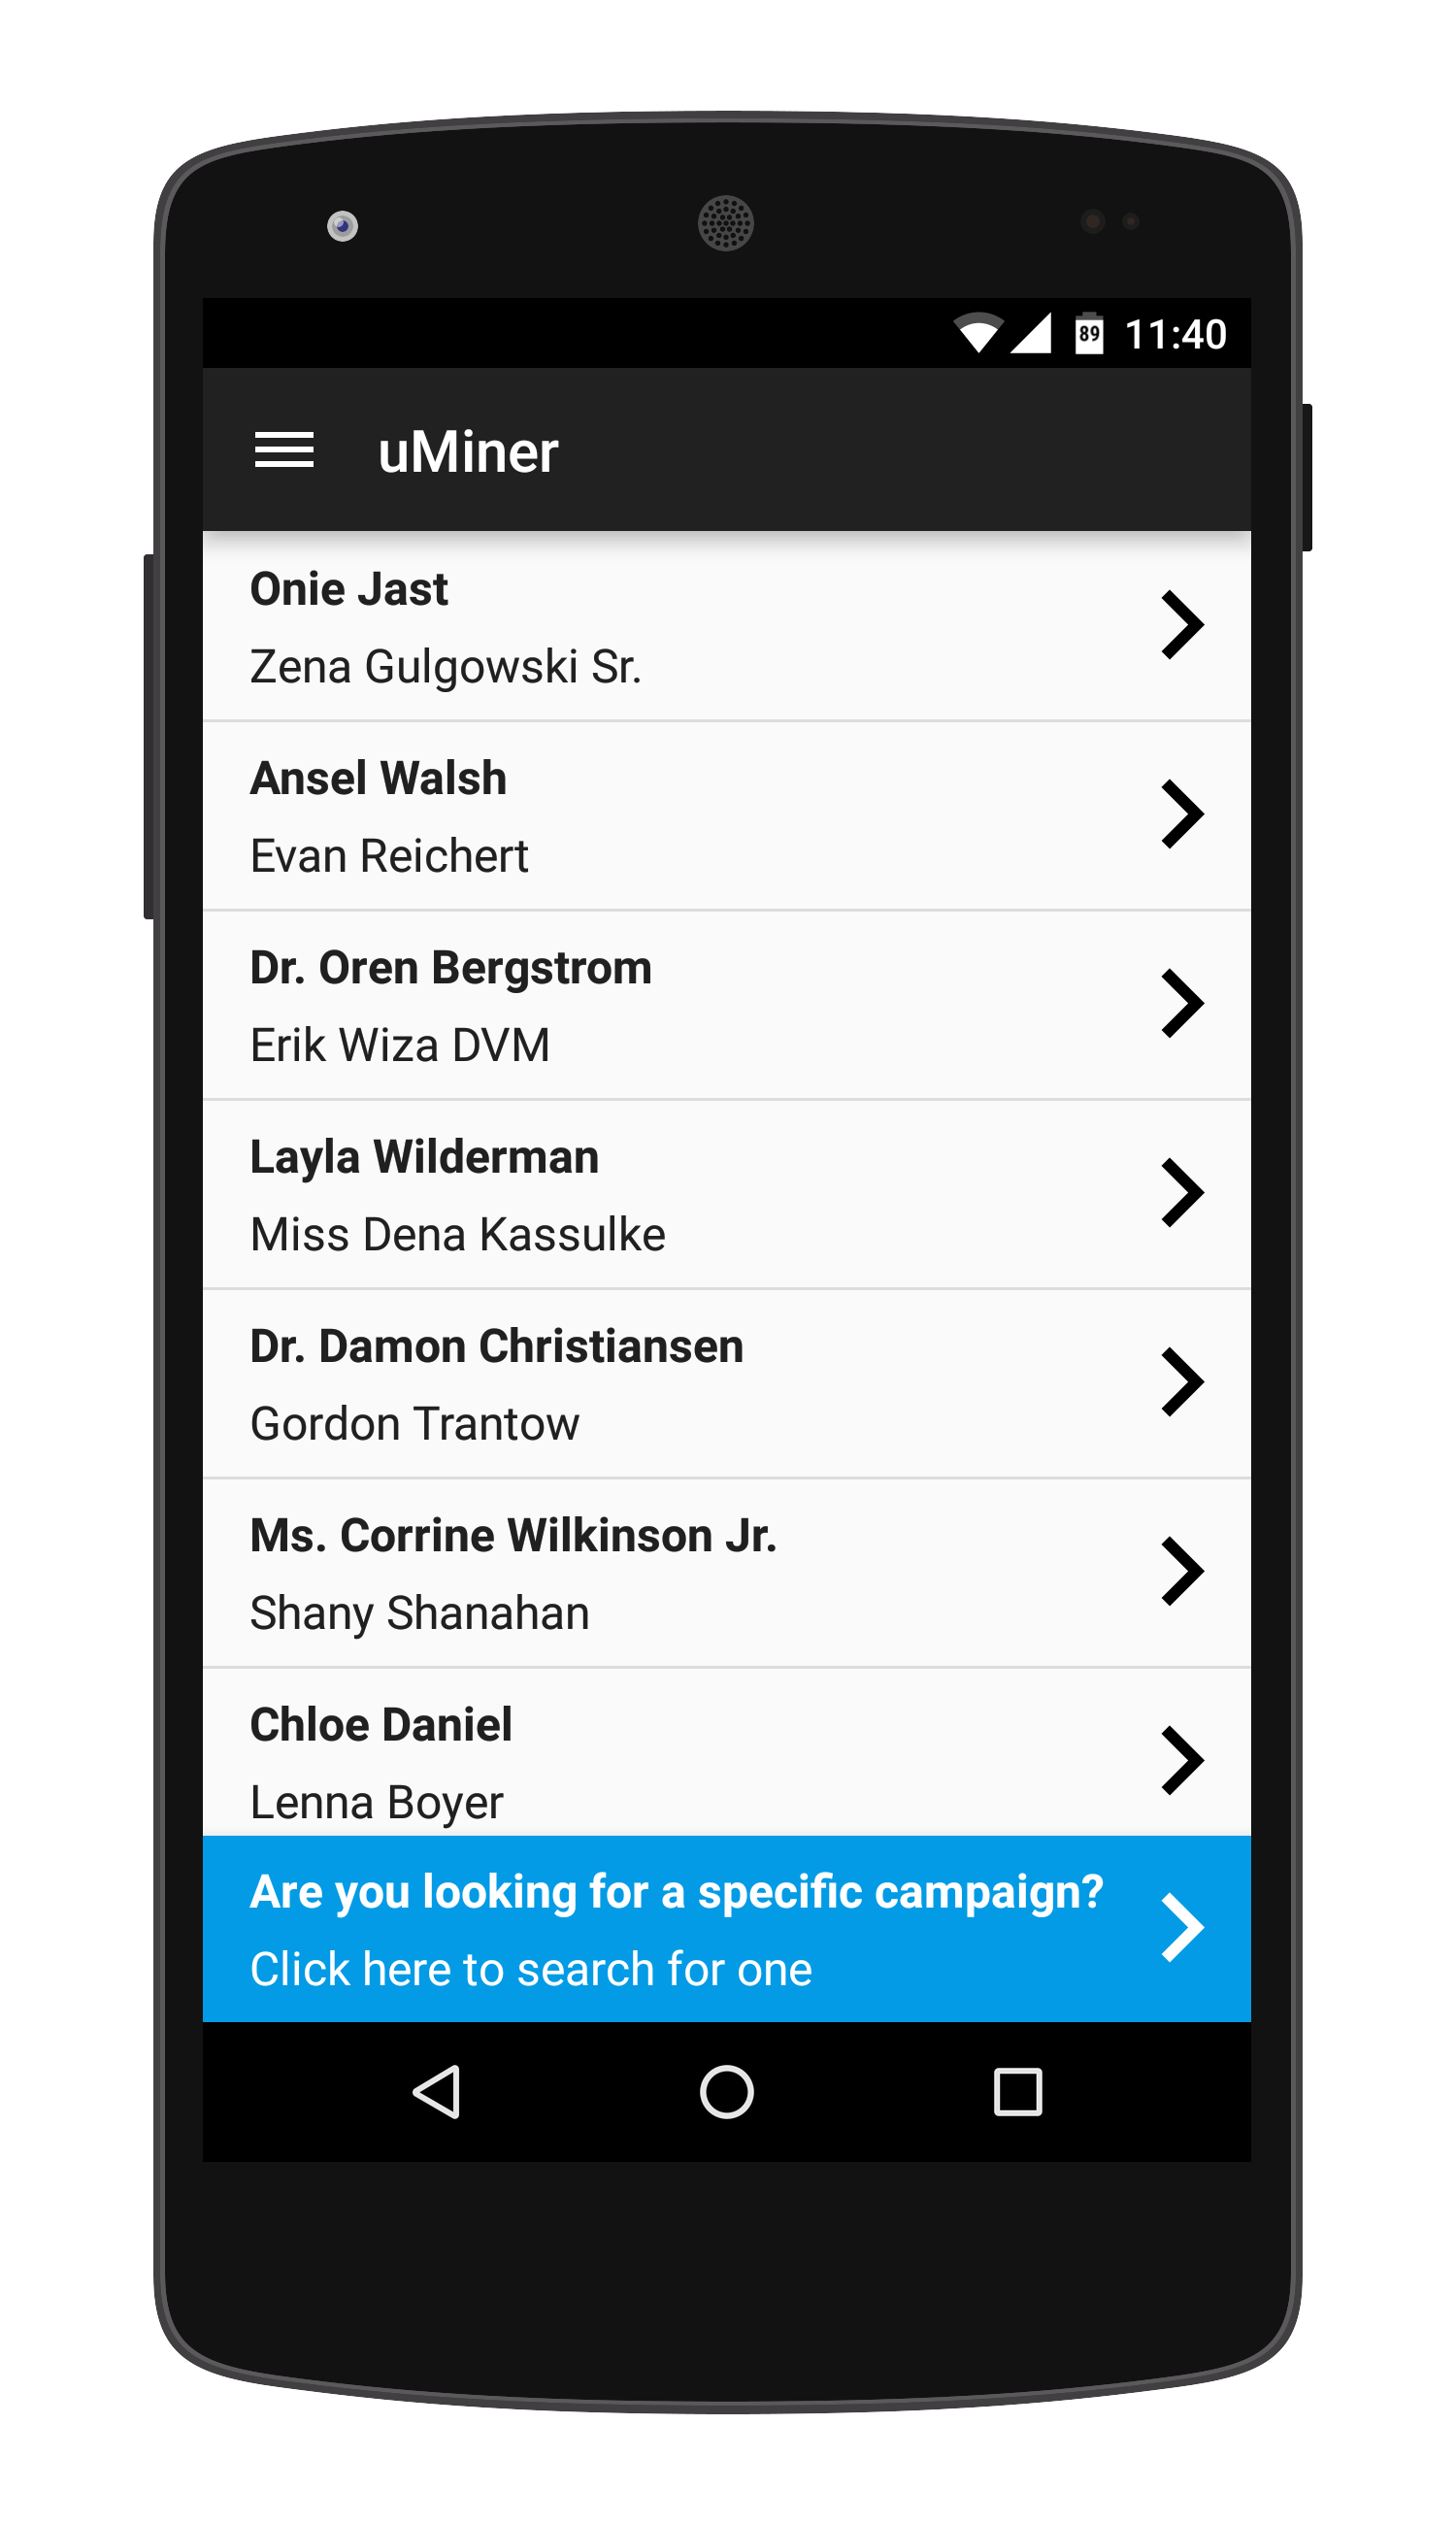
\includegraphics[width=.73\linewidth]{user_interfaces/client_public_campaigns_with_phone}
  \caption{Implementation.}
  \label{fig:implementation_public_campaigns}
\end{subfigure}
\caption{List of publicly available campaigns.}
\label{fig:public_campaigns}
\end{figure}
\FloatBarrier

An alternative way of finding campaigns, are through the view seen in \figref{fig:specific_campaign}. Here participants can enter a unique campaign identifier. If the identifier corresponds to a campaign, the participant will be redirected to a view similar to the one seen in \figref{fig:campaign_specification}. If not, he/she will be notified that the entered campaign identifier is invalid\todo{Dette afsnit skal ref til det sted hvor vi beskriver web-delen hvor man kan se hvilket ID campaignen har}. Throughout the project, we have thought of quite a number of different ways of allowing the participants to search for campaigns using different search criteria.

\begin{description}
 	\item[Quick Response Code (QR code)] could be utilized to give participants an easy way of subscribing to campaigns, simply by scanning a QR code. Customers would be able to distribute these QR codes through both digital and printed media. Furthermore, QR codes might be more easily relatable for participants, since they might be familiar with the concept from other domains.

 	\item[Specific search criteria] might help participants to find exactly what they want to contribute to. Participants might only want to contribute to campaigns with a scientific background, or campaigns that have next to no impact on battery life. Other criteria might be: limited amount of, or no questions in questionnaires; also some participants might not be willing to permit for specific sensors, so the possibility of searching for specific campaigns might be desirable.

 	\item[Prizes and other motivational factors] will potentially have a big impact on which campaigns gets contributed to. This means that the application could assist customers in getting more participants for their campaigns by displaying information regarding the prizes that customers might provide to willing participants. One could also imagine that participants could filter campaigns with or without prizes. 
\end{description} 


% Search for a campaign through a campaign identifier
\begin{figure}[!htbp]
\begin{subfigure}[!t]{.48\textwidth}
  \centering
  
\includegraphics[width=.7\linewidth]{mockups/join_specific_campaign}
  \caption{Mockup.}
  \label{fig:mockup_specific_campaign}
\end{subfigure}%
\begin{subfigure}[!t]{.52\textwidth}
  \centering
  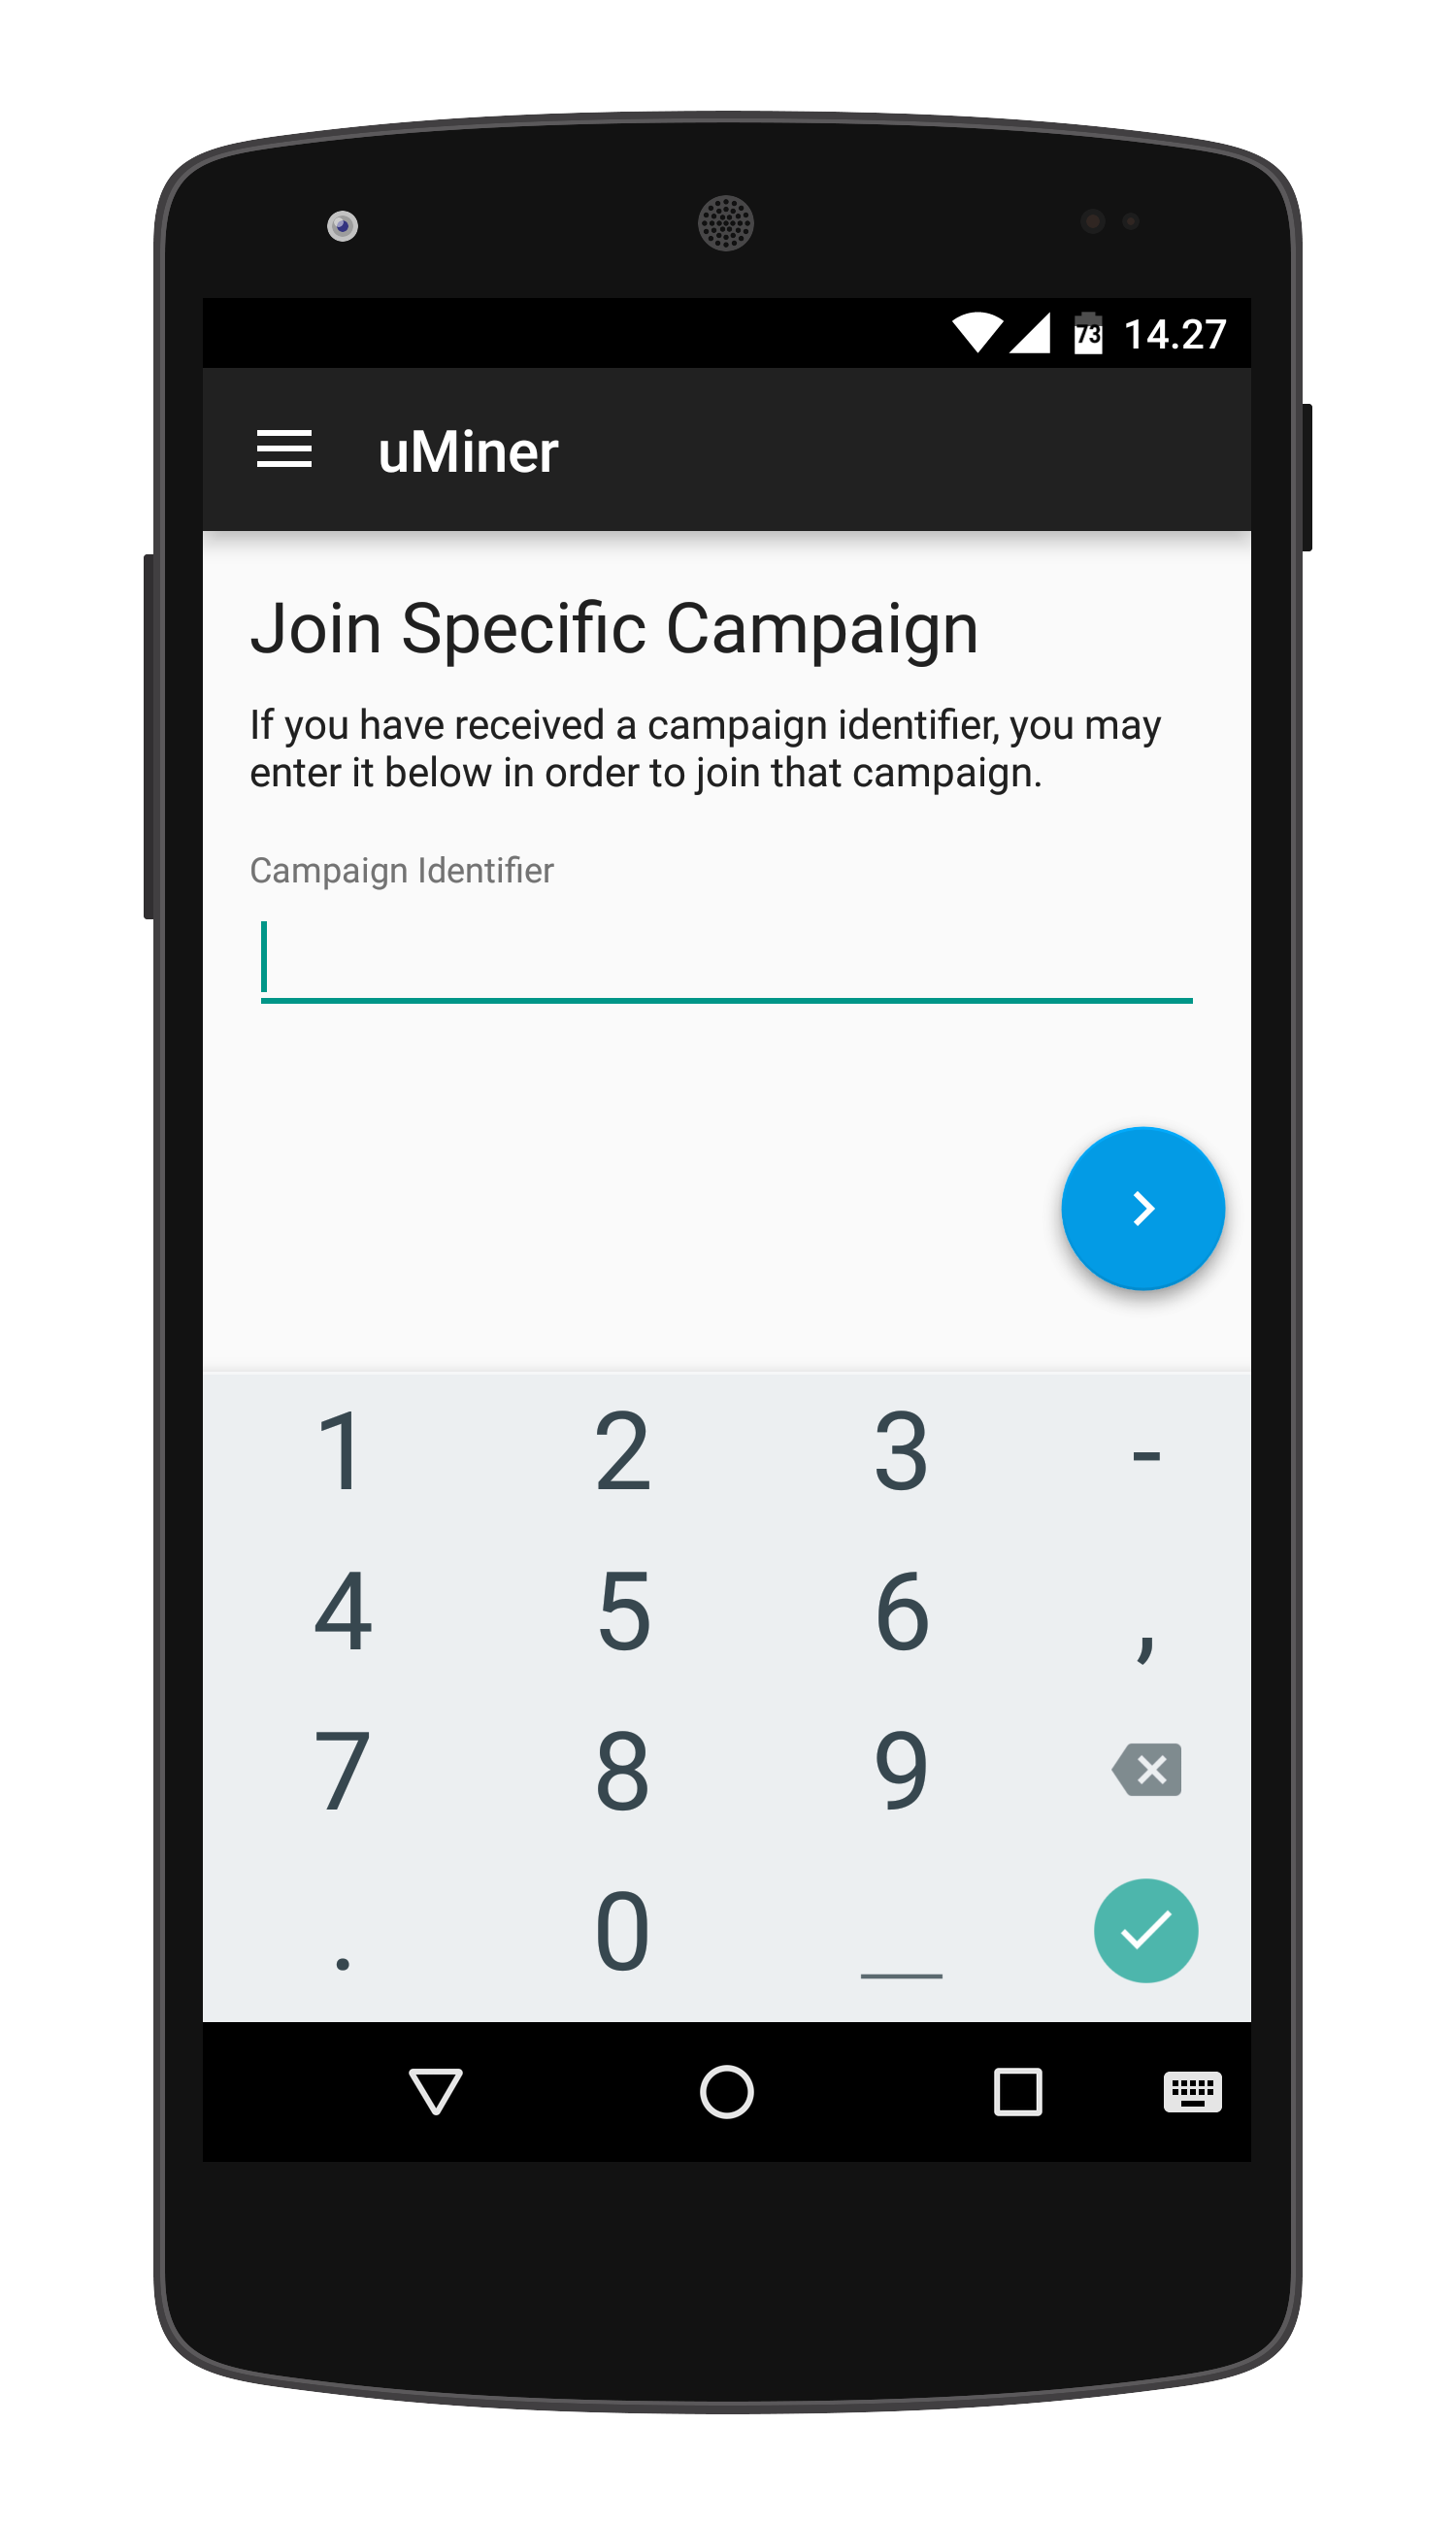
\includegraphics[width=.73\linewidth]{user_interfaces/client_join_specific_campaign_with_phone}
  \caption{Implementation.}
  \label{fig:implementation_specific_campaign}
\end{subfigure}
\caption{Search for a specific campaign using a campaign identifier.}
\label{fig:specific_campaign}
\end{figure}
\FloatBarrier

\subsection{Contributing to Campaigns}

% Campaign specification
\begin{figure}[!htbp]
\begin{subfigure}[!t]{.48\textwidth}
  \centering
  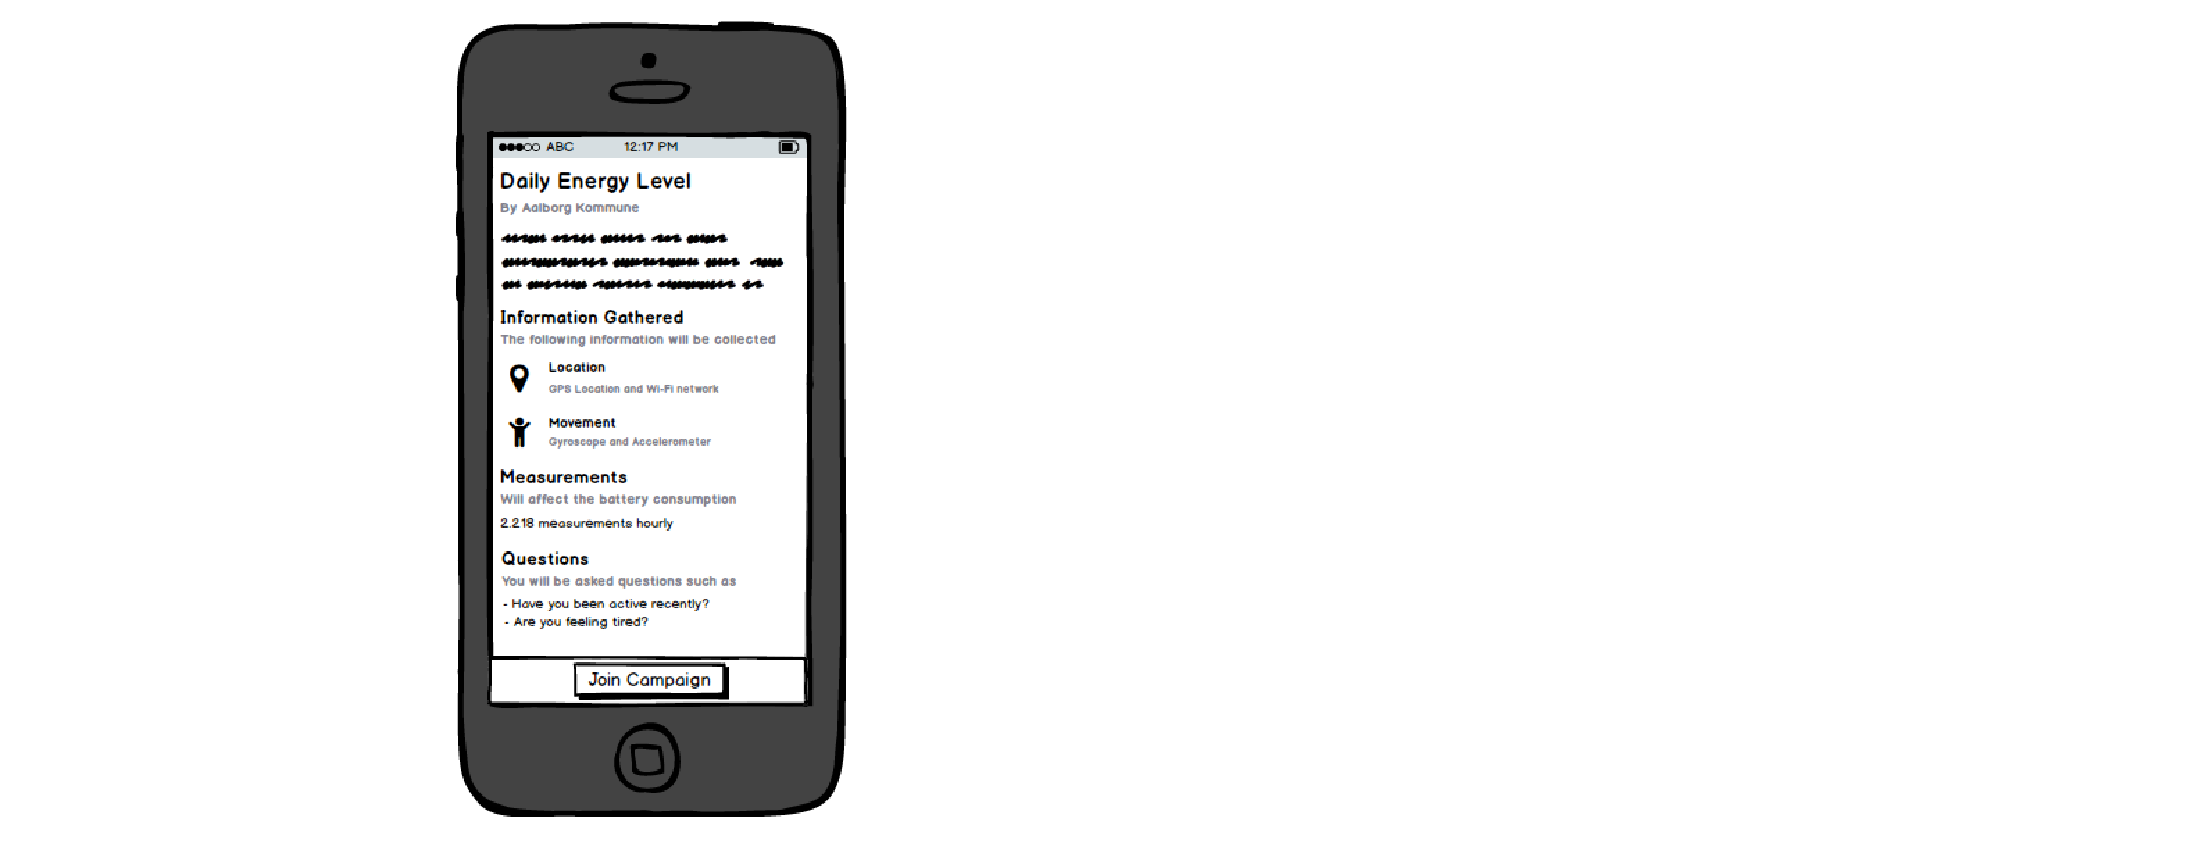
\includegraphics[width=.7\linewidth]{mockups/campaign_specification}
  \caption{Mockup.}
  \label{fig:mockup_campaign_specification}
\end{subfigure}%
\begin{subfigure}[!t]{.52\textwidth}
  \centering
  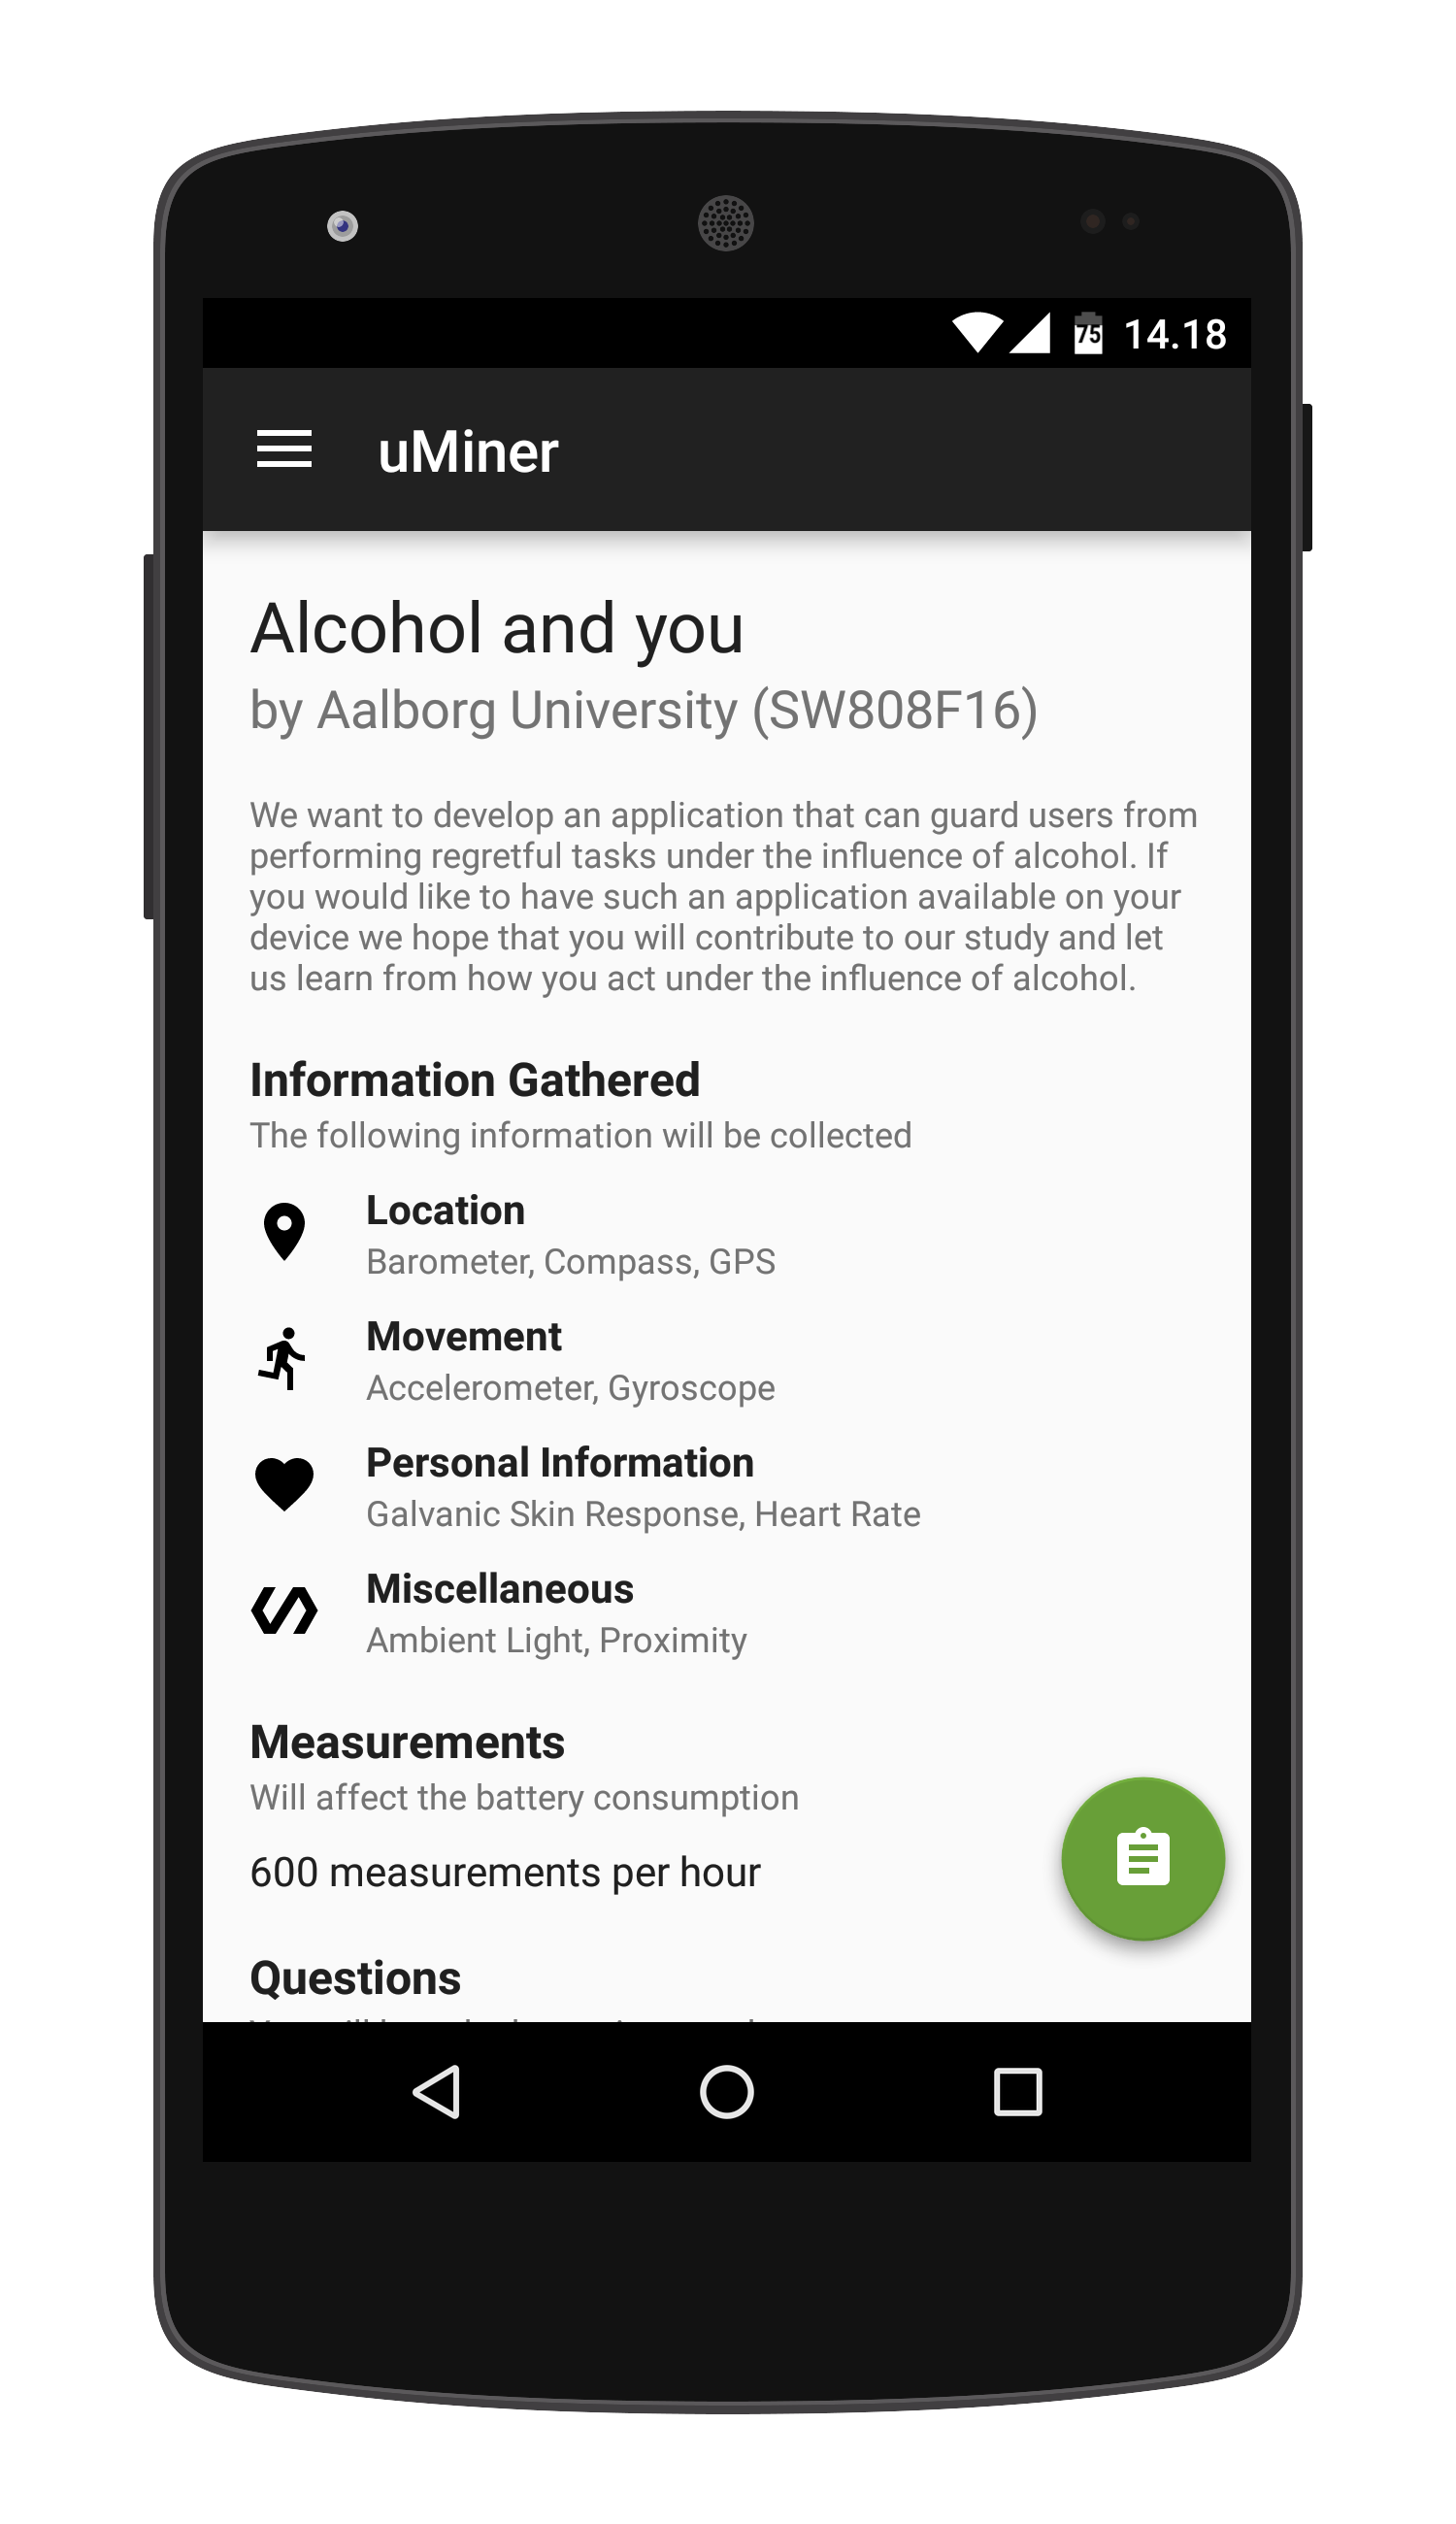
\includegraphics[width=.73\linewidth]{user_interfaces/client_campaign_specification2_with_phone}
  \caption{Implementation.}
  \label{fig:implementation_campaign_specification}
\end{subfigure}
\caption{Campaign specification view.}
\label{fig:campaign_specification}
\end{figure}
\FloatBarrier

% Leave campaign and dialog
\begin{figure}[!htbp]
\begin{subfigure}[!t]{.50\textwidth}
  \centering
  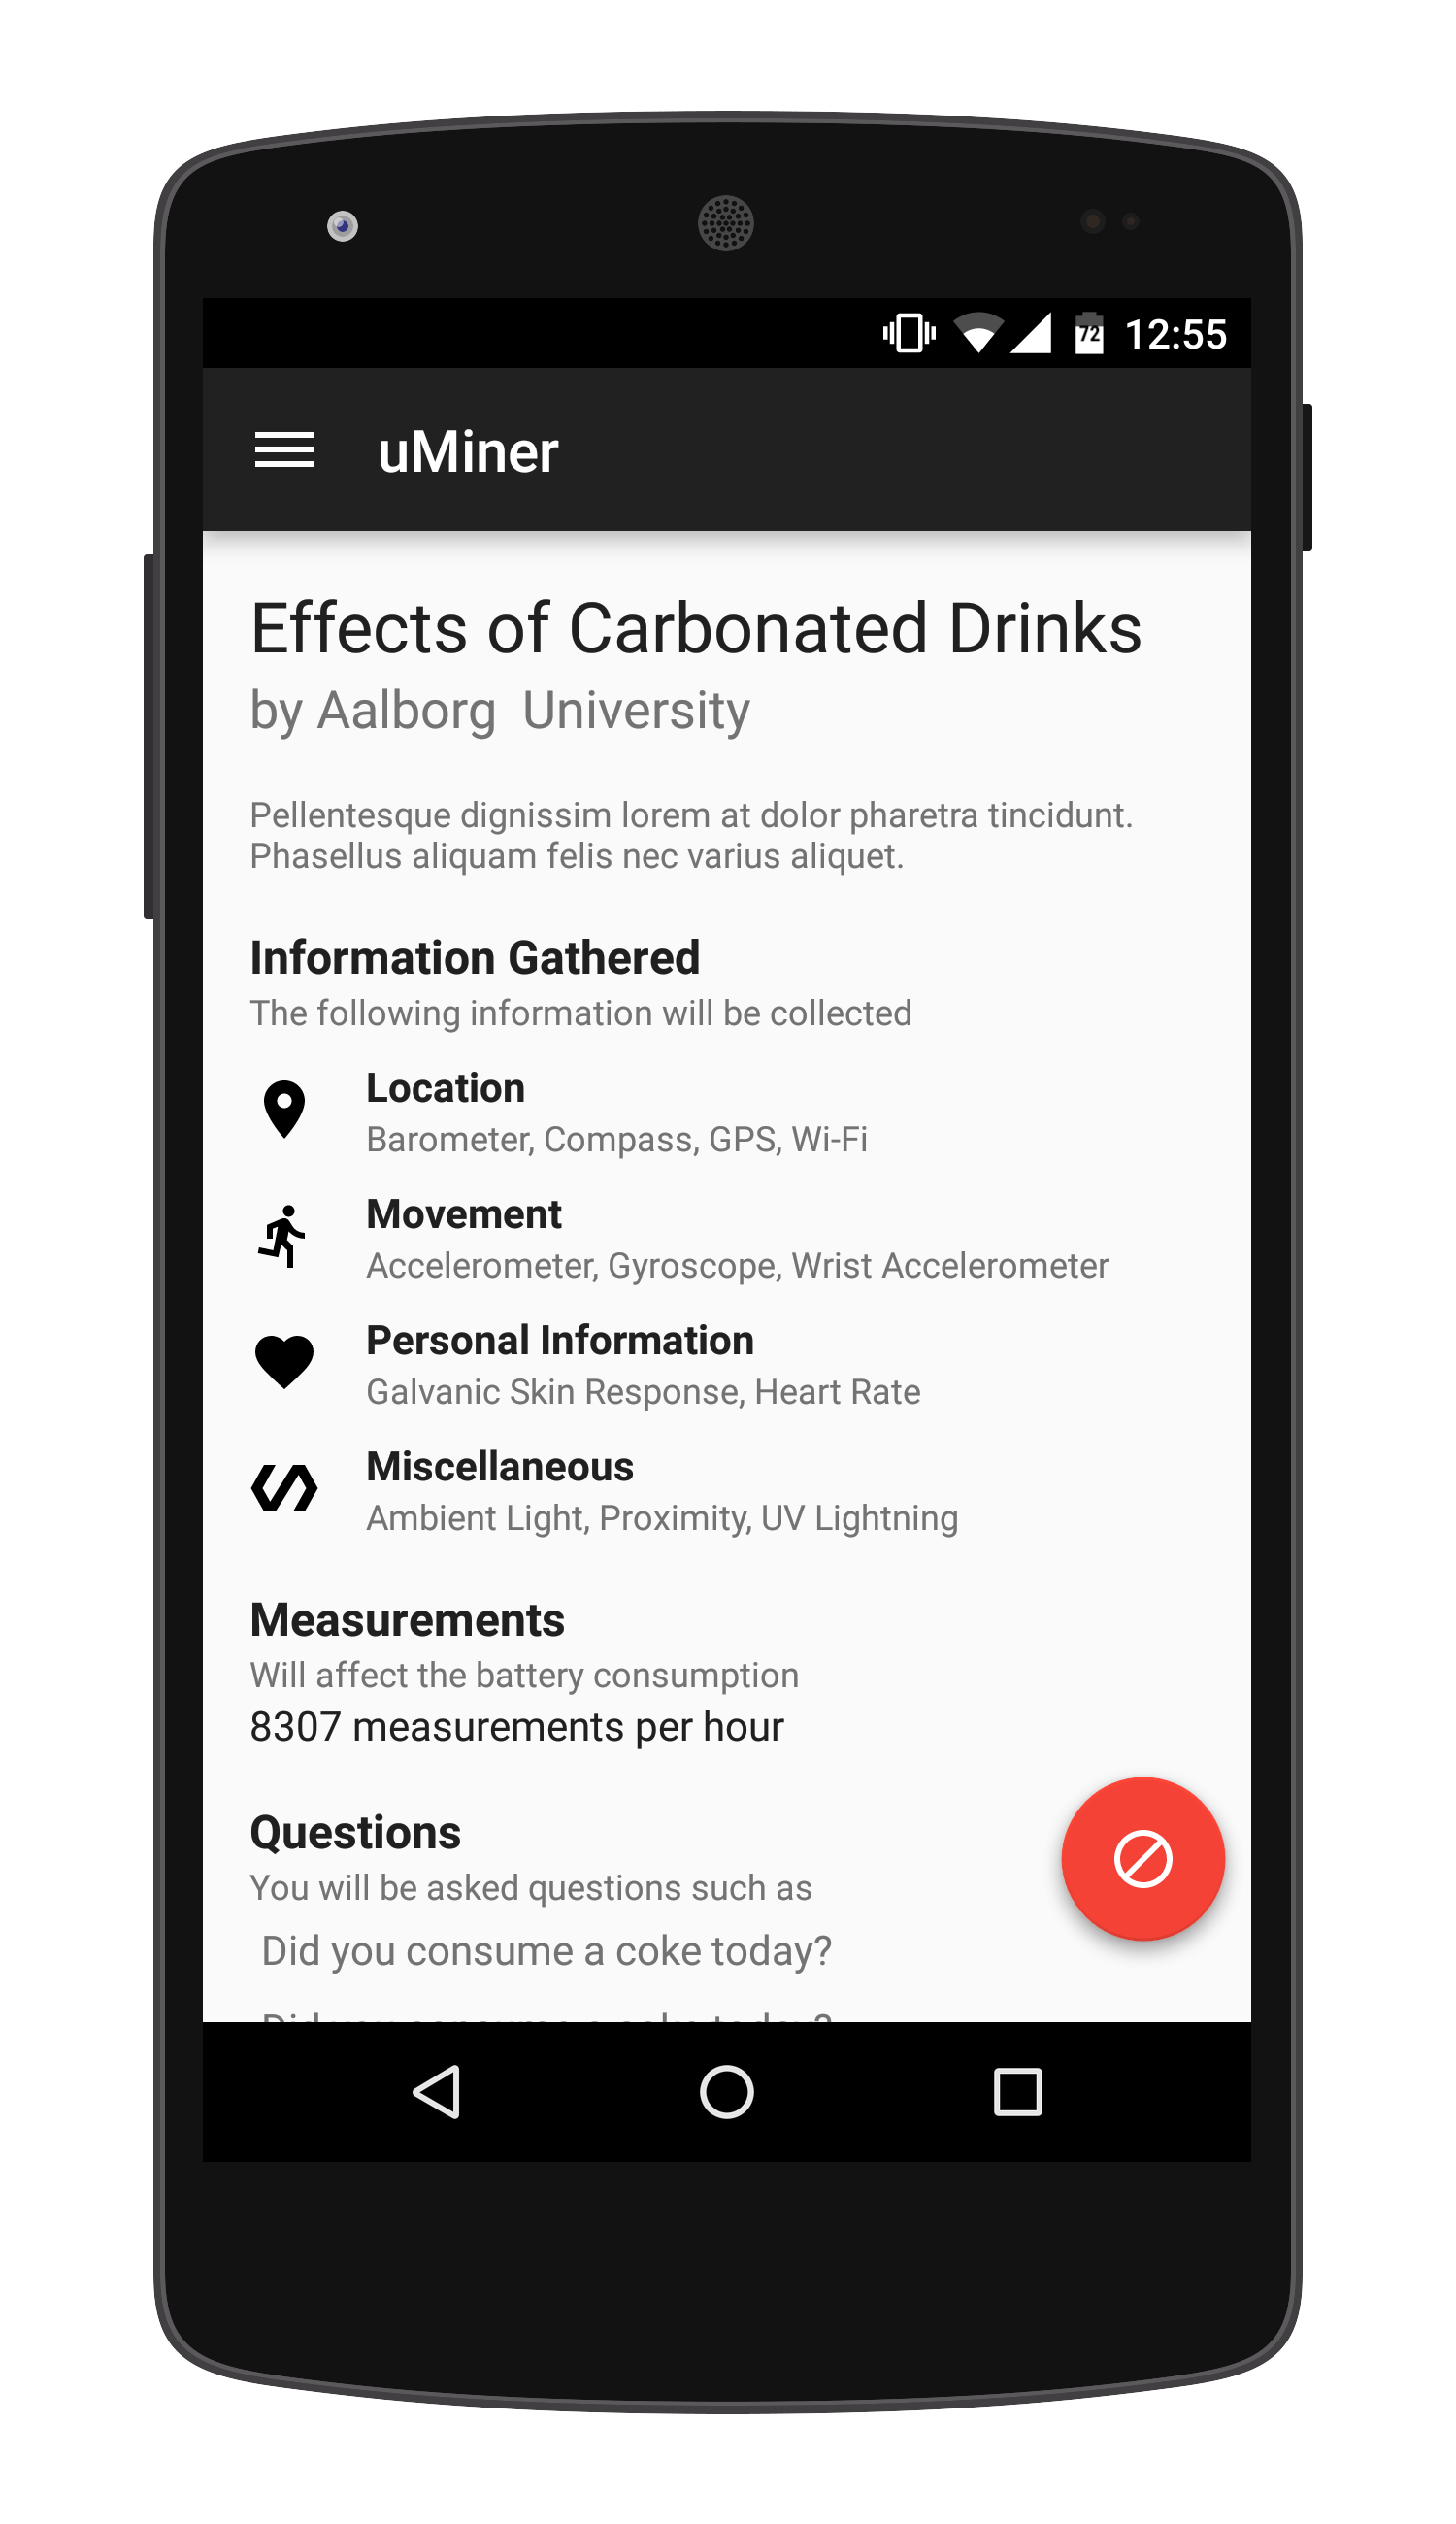
\includegraphics[width=.73\linewidth]{user_interfaces/client_leave_campaign_no_dialog_with_phone}
  \caption{Specification with leave button.}
  \label{fig:leave_campaign_no_dialog}
\end{subfigure}%
\begin{subfigure}[!t]{.50\textwidth}
  \centering
  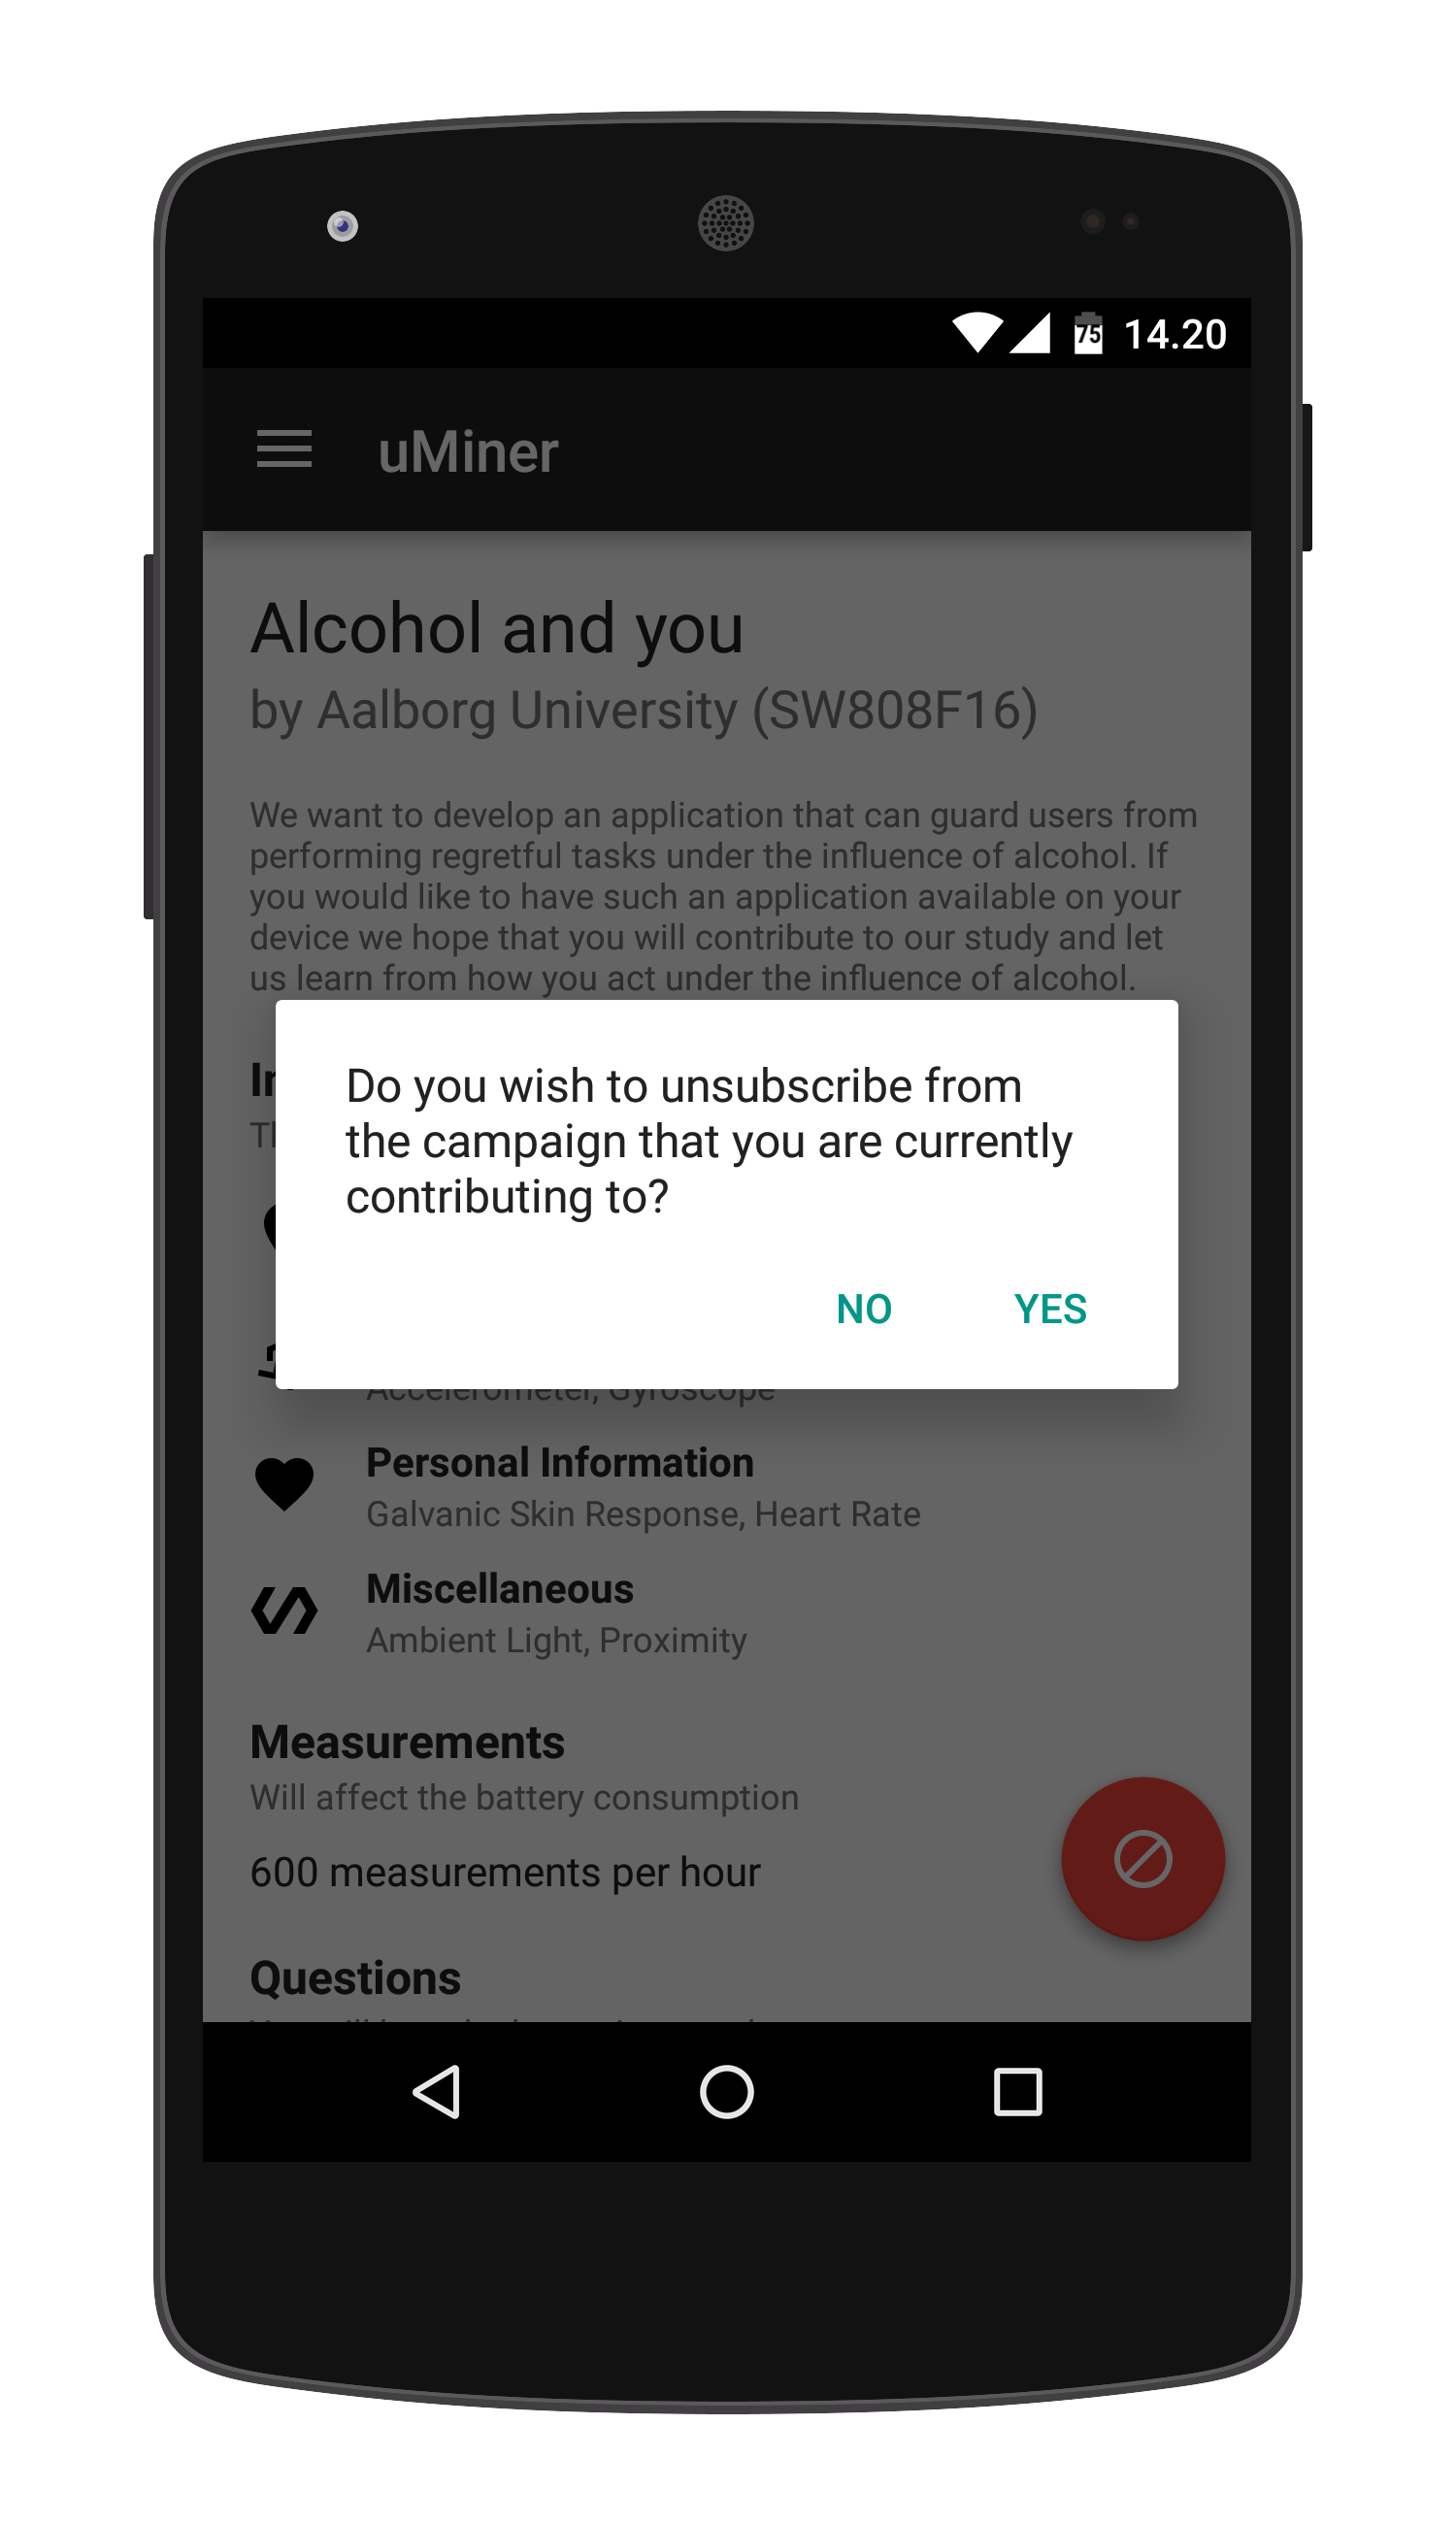
\includegraphics[width=.73\linewidth]{user_interfaces/client_leave_campaign_with_phone}
  \caption{Confirmation dialog.}
  \label{fig:leave_campaign_dialog}
\end{subfigure}
\caption{Leaving a campaign.}
\label{fig:leave_campaign}
\end{figure}
\FloatBarrier

\subsection{Answering Questionnaires}

% Answering questionnaires
\begin{figure}[!htbp]
\begin{subfigure}[!t]{.50\textwidth}
  \centering
  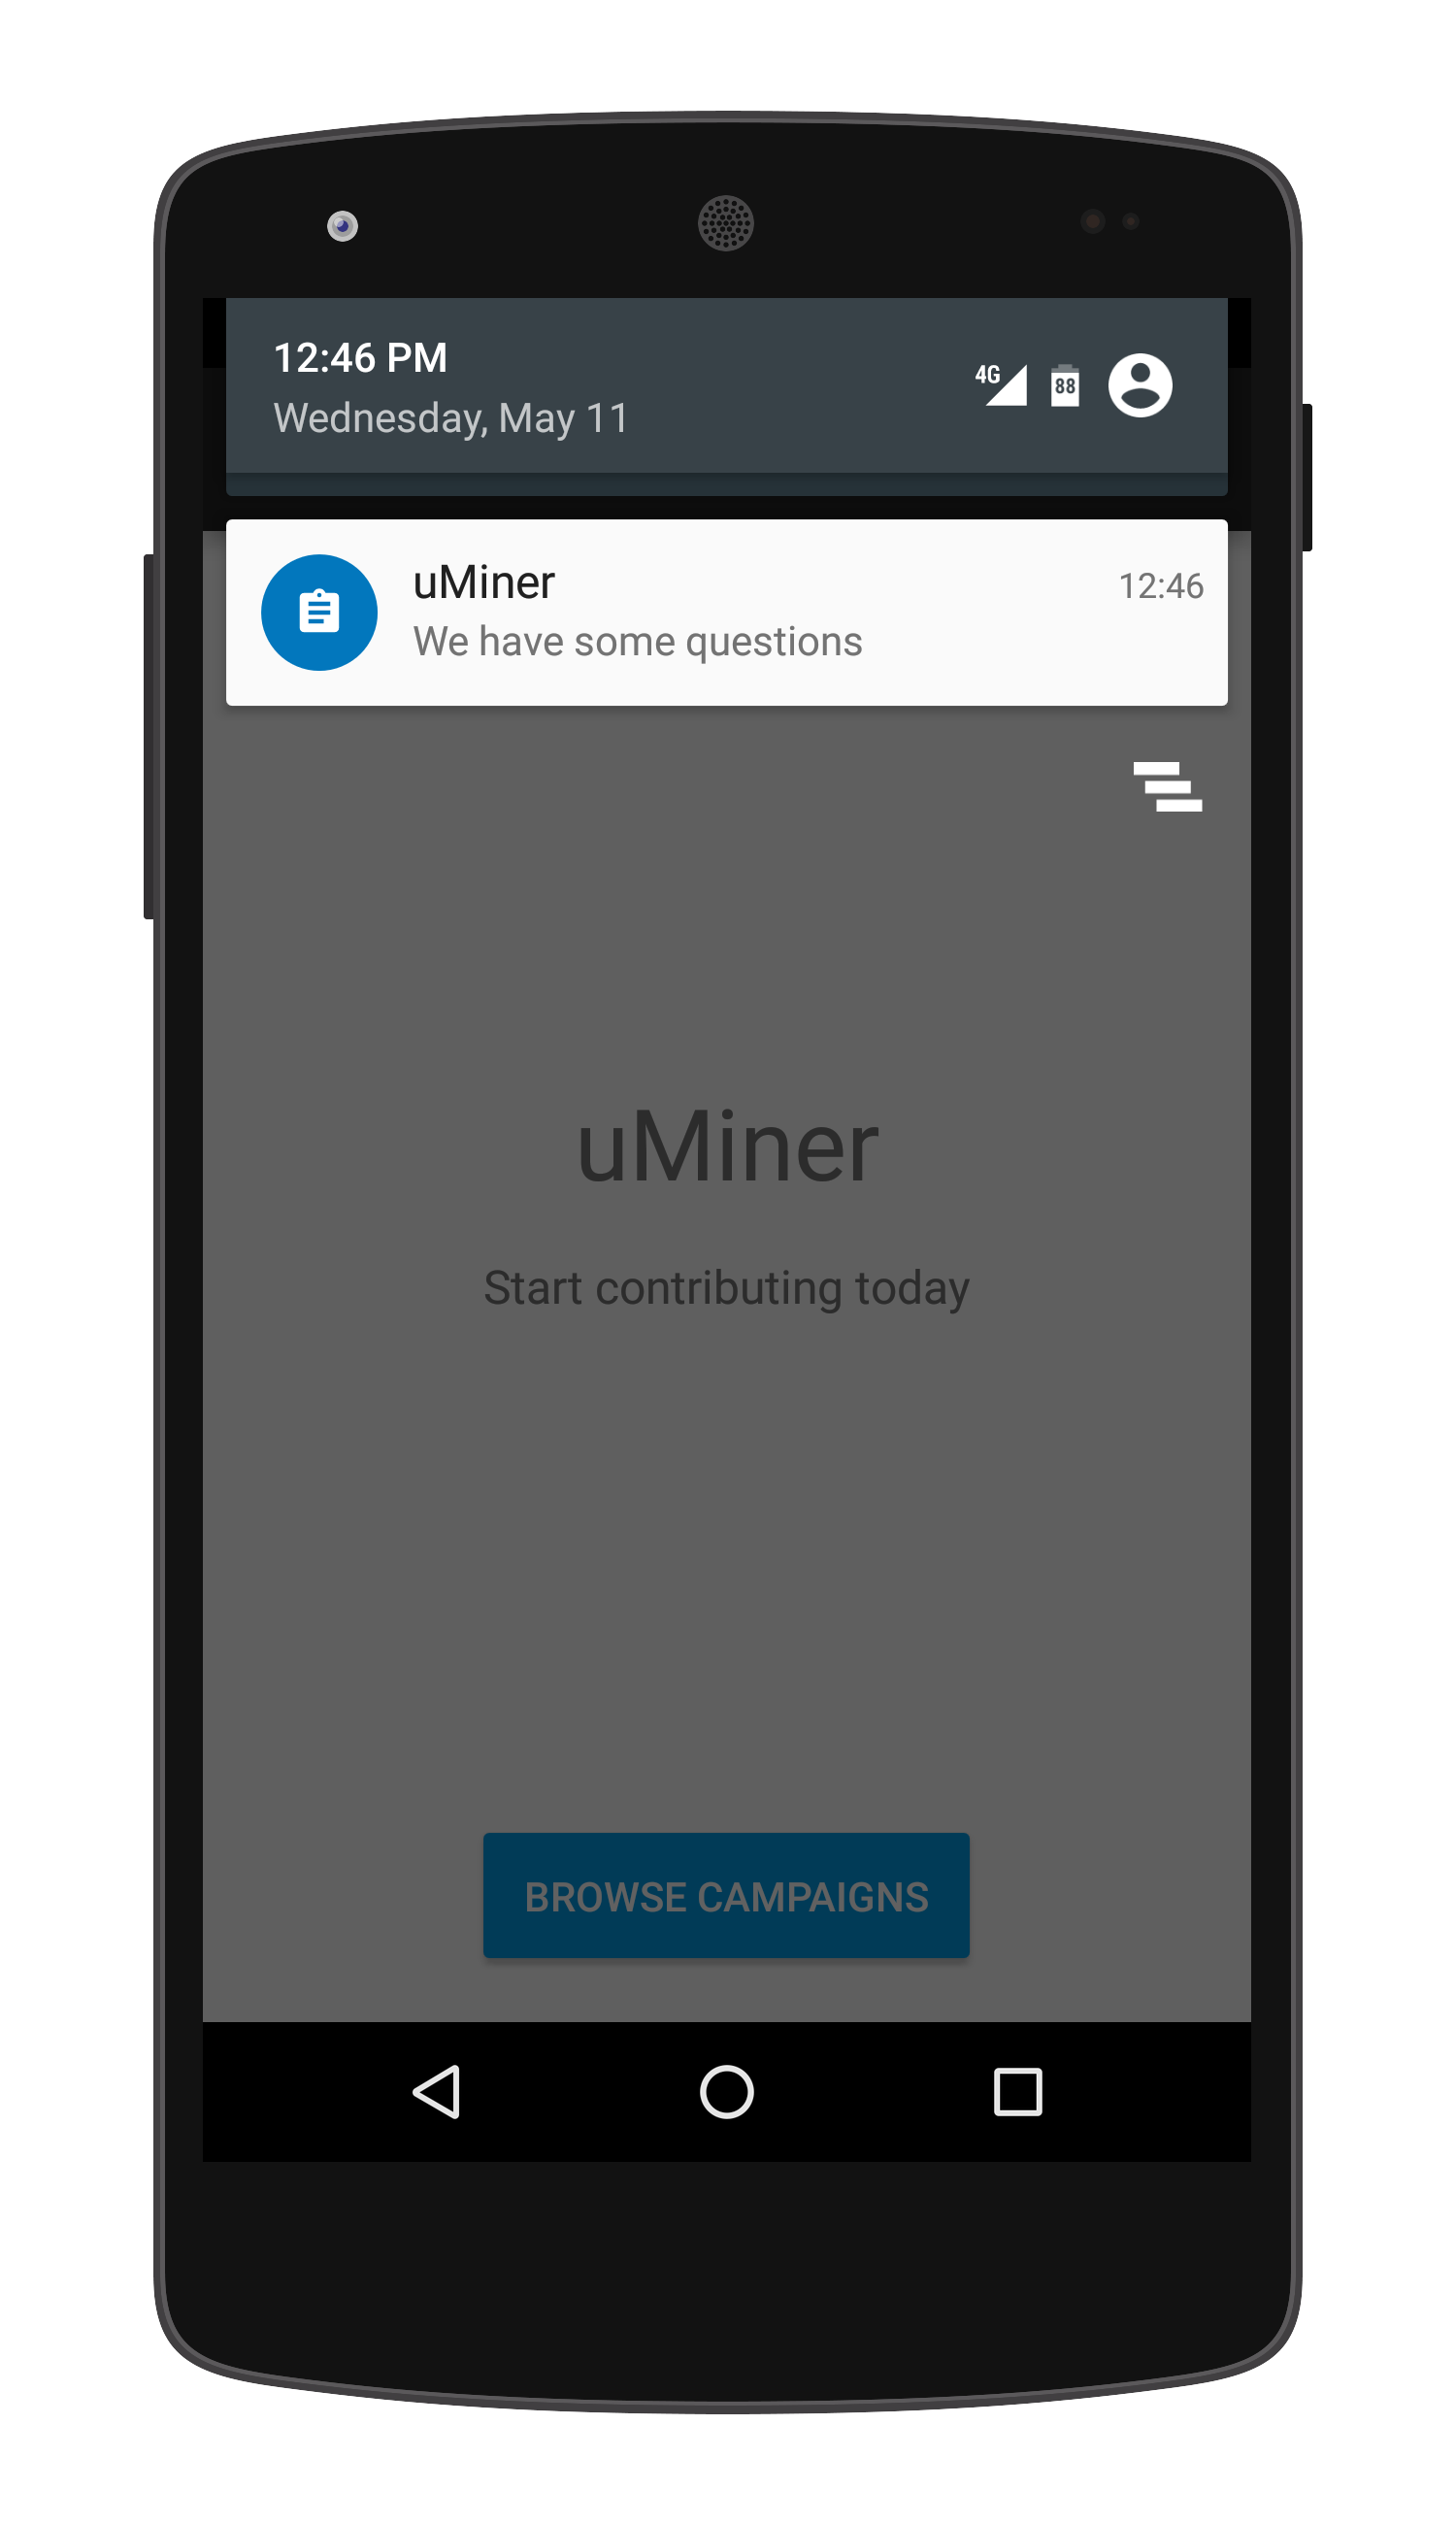
\includegraphics[width=.73\linewidth]{user_interfaces/client_notification_with_phone}
  \caption{Questionnaire notification.}
  \label{fig:answering_questionnaire_notification}
\end{subfigure}%
\begin{subfigure}[!t]{.50\textwidth}
  \centering
  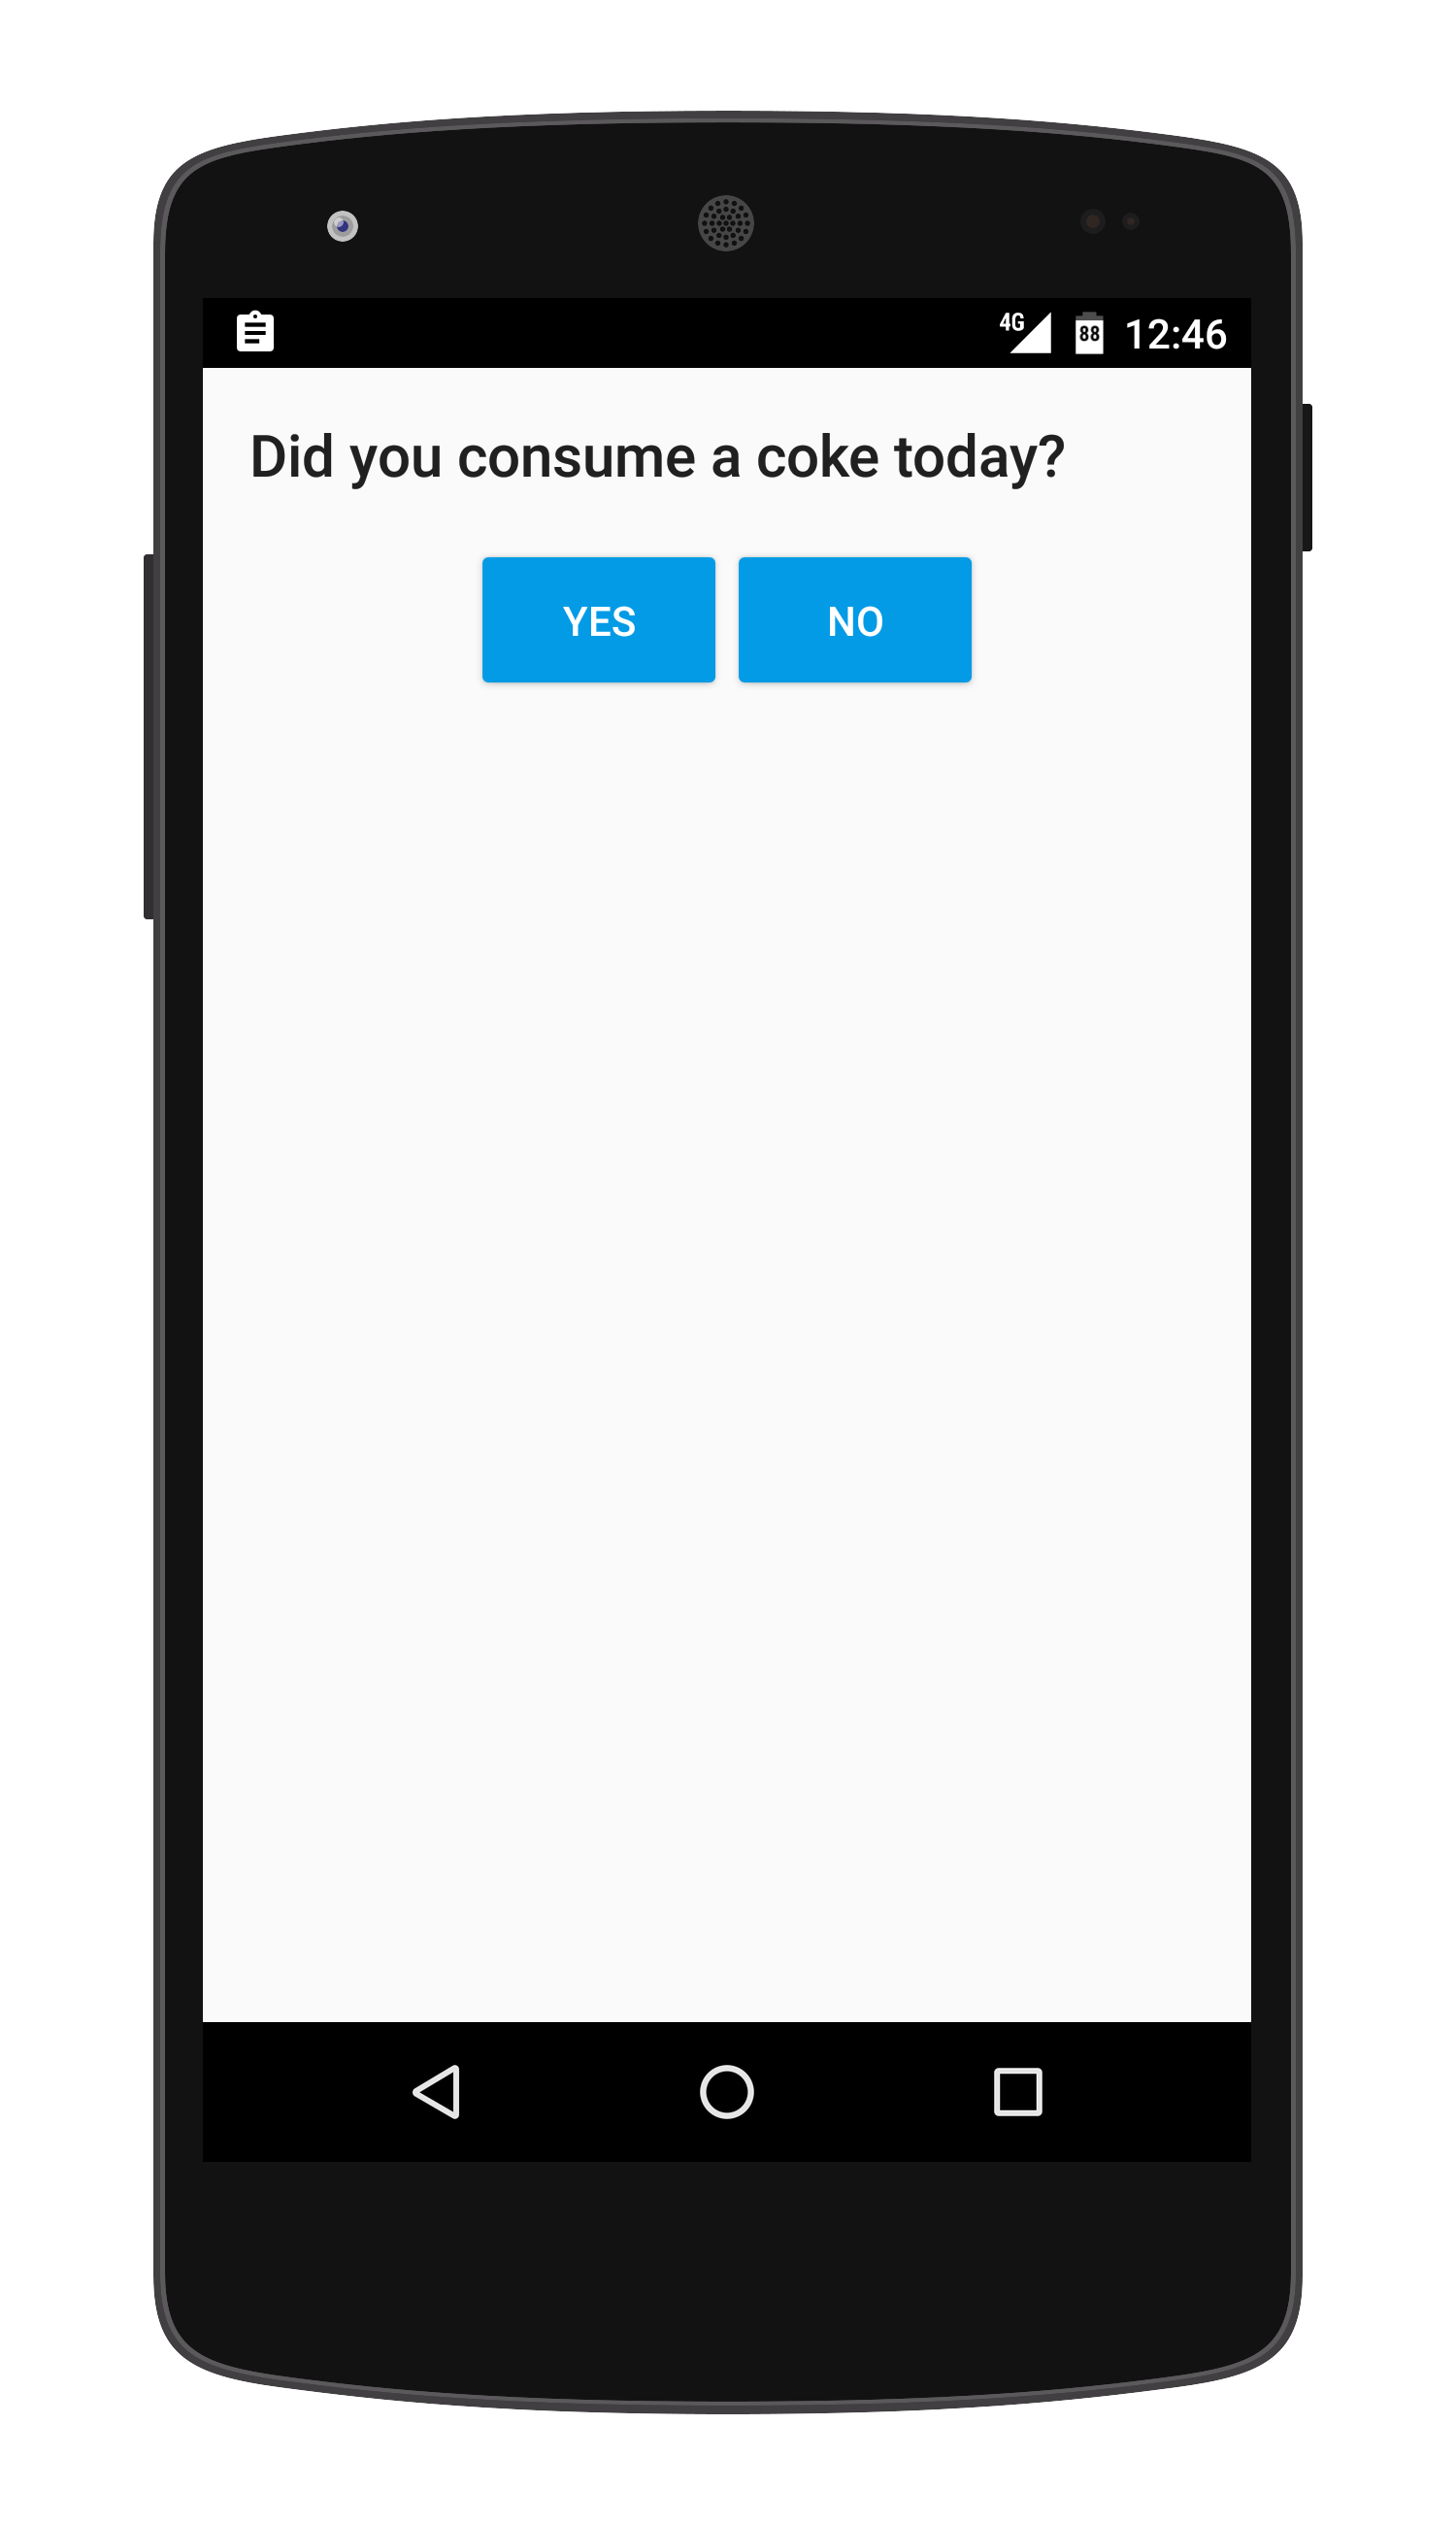
\includegraphics[width=.73\linewidth]{user_interfaces/client_answering_questions_with_phone}
  \caption{Answering the questionnaire.}
  \label{fig:answering_questionnaire_answering}
\end{subfigure}
\caption{Notification regarding questionnaire and answer view.}
\label{fig:answering_questionnaire}
\end{figure}
\FloatBarrier